\documentclass[conference]{IEEEtran}
\usepackage{graphicx,booktabs,amsmath,amssymb,url,xcolor,multirow}
\usepackage[hidelinks]{hyperref}
\graphicspath{{figures/}}
\newcommand{\repo}{\url{https://github.com/eman06/GenAI-A1}}
\newcommand{\video}{YouTube link to be added}

\begin{document}
\title{From Universal to Mixture-of-Experts Image Restoration, and Style-Conditioned Face-to-Sketch Synthesis:\\ Design, Evaluation and Deployment of Four Generative Models}
\author{\IEEEauthorblockN{Eman Ihsan}\IEEEauthorblockA{Generative AI, Assignment 1\\Code: \repo\quad Demo: \video}}
\maketitle

\begin{abstract}
We build and deploy four related generative systems. On the Oxford-IIIT Pet dataset with runtime-generated salt-and-pepper noise, Gaussian blur and rectangular occlusion, we compare (i) a single universal denoising autoencoder (UDAE), (ii) a corruption classifier that hard-routes inputs to three specialist autoencoders with an identity bypass for clean images, and (iii) a jointly fine-tuned soft mixture-of-experts (MoE) whose gate is initialised from the classifier. On FS2K we train (iv) a pix2pix-style conditional GAN whose U-Net generator and PatchGAN discriminator are both conditioned on a learned sketch-style embedding. Every model is tuned with Optuna, tracked with MLflow, exported to ONNX (verified against PyTorch to $<10^{-6}$ max absolute error), and served by a FastAPI + React application started with one Docker Compose command. On 36{,}690 test cases the classifier routes 99.71\% of inputs correctly, hard routing raises mean PSNR from 22.33\,dB (corrupted input) to 27.46\,dB versus 22.19\,dB for the universal DAE, and the jointly trained soft MoE reaches the best SSIM (0.832) while assigning more than 0.9 weight to a single branch for 88\% of images. The style-conditioned cGAN produces visibly different sketch styles from the same photograph and reaches a test SSIM of 0.58 / 0.47 / 0.35 for styles 3 / 1 / 2 (Style~2, dense pencil hatching, is the hardest).
\end{abstract}

\section{Introduction}
Real images are degraded in heterogeneous ways, and a single restoration network must trade capacity between incompatible inverse problems: removing impulse noise requires discarding isolated outliers, de-blurring requires amplifying high frequencies, and inpainting requires hallucinating plausible content. We study three ways of organising this capacity, a shared model, hard specialisation, and soft specialisation, under one controlled corruption protocol, and complement them with a paired image-to-image GAN. The emphasis is on evidence: each design decision is backed by an ablation, an Optuna study, or a cited prior result.

\section{Related Work}
Denoising autoencoders learn robust representations by reconstructing clean inputs from corrupted ones~\cite{vincent2008}; convolutional encoder-decoders with symmetric skips are strong restorers~\cite{mao2016}, but unrestricted skips can bypass the bottleneck, which the assignment forbids. Combining an L1 term with SSIM produces sharper, perceptually better restorations than L2 alone~\cite{zhao2017}. Mixture-of-experts models route inputs to specialised sub-networks through a learned gate~\cite{jacobs1991}; sparsely-gated MoEs add load-balancing terms to prevent the gate from collapsing onto a few experts~\cite{shazeer2017,fedus2022}, which motivates our balance regulariser. Conditional GANs for paired translation (pix2pix) combine an adversarial PatchGAN loss with an L1 reconstruction term weighted by $\lambda=100$~\cite{isola2017}; class-conditioning through learned embeddings follows~\cite{mirza2014,miyato2018}. FS2K~\cite{fan2022} provides 2{,}104 photo--sketch pairs in three styles. Hyper-parameters are optimised with the TPE sampler and median pruning of Optuna~\cite{akiba2019}.

\section{Data and Corruption Protocol (Tasks 1--3)}
The official Oxford-IIIT Pet \emph{trainval} split (3{,}680 images) is divided 80/20 with seed 42 into 2{,}944 training and 736 validation images; the 3{,}669-image \emph{test} split is only touched by the final evaluation scripts. Images are converted to RGB and resized to $128\times128$ (bicubic).
\textbf{Runtime corruption.} Corruption happens inside the DataLoader's collate function, so every time an image is loaded a new condition and severity are drawn and nothing is written to disk. Task~1 draws each image's condition uniformly from \{clean, salt-and-pepper, blur, occlusion\}; Tasks~2--3 build exactly class-balanced batches. Salt-and-pepper replaces a fraction $p\sim\mathcal U(0.02,0.15)$ of pixels by black or white (50/50); blur uses $k\in\{3,5,7\}$, $\sigma\sim\mathcal U(0.5,2.5)$; occlusion inserts 1--3 non-overlapping black rectangles jointly covering $\mathcal U(10\%,35\%)$ of the image (Dirichlet area split, log-uniform aspect ratio in $[\frac12,2]$).
\textbf{Deterministic validation/test.} A validation manifest stores one fixed corruption (type, parameters, rectangle coordinates, seed) per validation image. The test manifest stores, for every test image, the clean input plus three corruptions at three fixed severities ($p\in\{0.03,0.08,0.15\}$; $(k,\sigma)\in\{(3,0.7),(5,1.5),(7,2.5)\}$; 1/2/3 rectangles covering $\approx$10/20/35\%), i.e.\ 36{,}690 test cases. The corruption code is pure NumPy and is imported unchanged by the web backend, so the app reproduces the exact test conditions. Unit tests check every range, the 50/50 salt/pepper split, occlusion coverage, determinism, and that our separable blur matches \texttt{torchvision} to $10^{-5}$.
\textbf{Metrics.} PSNR (capped at 50\,dB: an identity output on a clean input would otherwise give $\approx$100\,dB and dominate averages), SSIM (11$\times$11 Gaussian window) and L1, always against the clean target.

\section{Task 1: Universal Denoising Autoencoder}
\subsection{Architecture}
Fig.~\ref{fig:t1arch}: three stride-2 convolutional stages (channels $b,2b,4b$) reduce $128^2$ to $16^2$; a $1\times1$ convolution produces a $16\times16\times c$ latent ($c\in\{4,8,16,32\}$, i.e.\ 12--48$\times$ fewer values than the 49{,}152-value input). A mirrored decoder with transposed convolutions and a sigmoid output reconstructs the RGB image. There are \emph{no} skip connections, so all information passes through the bottleneck. Dropout2d is applied in the encoder and at the latent.
\IfFileExists{figures/t1_udae.png}{\begin{figure}[t]\centering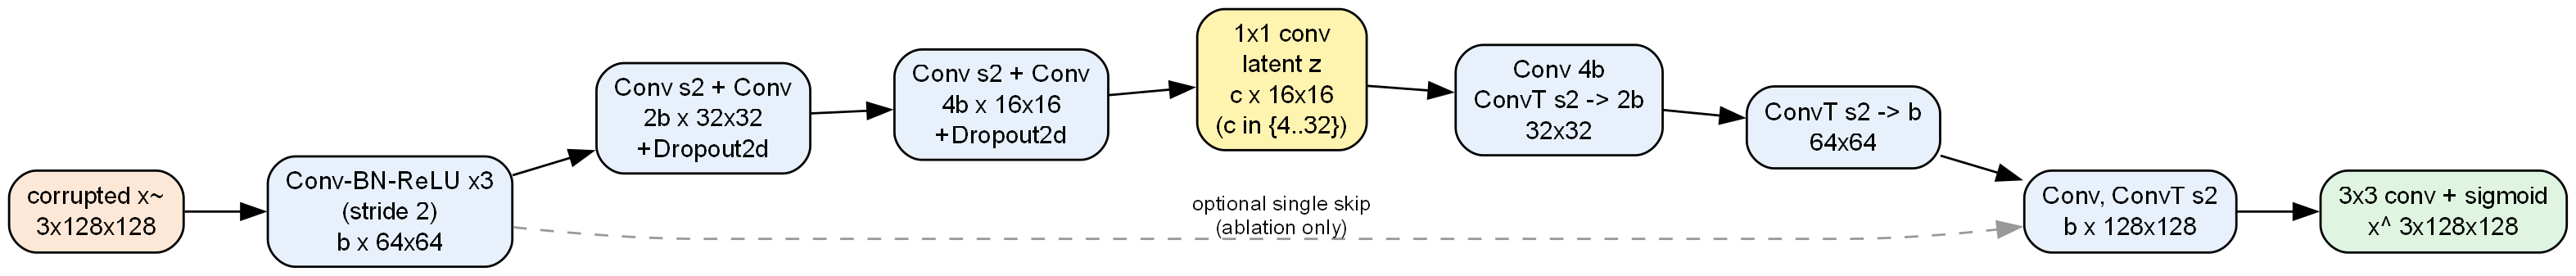
\includegraphics[width=\linewidth]{t1_udae.png}\caption{Universal DAE. The dashed skip exists only in the ablation.}\label{fig:t1arch}\end{figure}}{}
\subsection{Loss and Optuna search}
$\mathcal L_{UDAE}=\alpha\,\mathcal L_{1}(x,\hat x)+(1-\alpha)(1-\mathrm{SSIM}(x,\hat x))$, with SSIM computed in fp32 because it was numerically unstable under mixed precision. Optuna (TPE, seed 42, median pruner after 2 epochs, 12 trials $\times$ 6 epochs) searched lr $\in[10^{-4},3\cdot10^{-3}]$ (log), batch $\in\{16,32,64\}$, latent channels $\in\{4,8,16,32\}$, base channels $\in\{16,32,48,64\}$, dropout $\in[0,0.3]$ and $\alpha\in[0.5,0.95]$; the first trial was the suggested starting point ($\alpha=0.8$). \emph{Key design choice:} the objective is validation $\mathcal L_1+(1-\mathrm{SSIM})$ with \emph{fixed} equal weights. Scoring each trial with its own $\alpha$-weighted loss would make trials incomparable and bias the search towards whichever $\alpha$ makes its own loss numerically smallest. Of 12 trials, 8 were pruned by the median rule. The best trial used lr $3.6\cdot10^{-4}$, batch 16, latent $16{\times}16{\times}32$ (6$\times$ compression), 64 base channels, dropout 0.25 and $\alpha=0.60$ (validation SSIM 0.738 after 6 epochs). Optuna moved $\alpha$ well below the suggested 0.8: once trials are scored on a fixed scale, a larger SSIM share is preferred. The parameter-importance plot ranks latent size and learning rate first, consistent with bottleneck capacity limiting reconstruction more than regularisation does. The best configuration was retrained for 35 epochs (AdamW, one-cycle LR, AMP).
\subsection{Results}
\begin{table}[t]\centering\caption{Task 1 universal DAE on the official test set (3{,}669 images per condition). PSNR in dB, capped at 50.}\label{tab:t1}\setlength{\tabcolsep}{4pt}
\begin{tabular}{llrrrr}\toprule
Input & Sev. & PSNR$_{in}$ & PSNR$_{out}$ & SSIM$_{in}$ & SSIM$_{out}$\\ \midrule
Clean & none & 50.00 & 23.29 & 1.000 & 0.849 \\
S\&P & low & 20.13 & 23.27 & 0.602 & 0.846 \\
S\&P & medium & 15.87 & 23.20 & 0.340 & 0.837 \\
S\&P & high & 13.14 & 23.00 & 0.204 & 0.819 \\
Blur & low & 32.34 & 23.37 & 0.944 & 0.846 \\
Blur & medium & 26.77 & 23.02 & 0.806 & 0.816 \\
Blur & high & 24.35 & 21.92 & 0.692 & 0.711 \\
Occl. & low & 16.70 & 21.59 & 0.862 & 0.796 \\
Occl. & medium & 13.27 & 20.38 & 0.726 & 0.743 \\
Occl. & high & 10.75 & 18.90 & 0.536 & 0.663 \\
\bottomrule\end{tabular}\end{table}
\begin{table*}[t]\centering\caption{Comparison of the three restoration systems on the same 36{,}690 test cases (PSNR in dB).}\label{tab:cmp}
\begin{tabular}{lrrrrrr}\toprule
System & Clean & S\&P & Blur & Occlusion & Overall PSNR & Overall SSIM\\ \midrule
Soft MoE (T3) & 48.69 & 26.90 & 26.43 & 22.03 & 27.48 & 0.832 \\
Universal DAE (T1) & 23.29 & 23.16 & 22.77 & 20.29 & 22.19 & 0.792 \\
Hard routing, predicted (T2) & 49.83 & 26.71 & 26.10 & 22.11 & 27.46 & 0.821 \\
Hard routing, oracle (T2) & 50.00 & 26.71 & 26.10 & 22.12 & 27.48 & 0.821 \\
\bottomrule\end{tabular}\end{table*}
Table~\ref{tab:t1} reports test performance by corruption and severity, and Fig.~\ref{fig:t1ex} shows examples. The universal DAE is strongly beneficial when the input is badly damaged: salt-and-pepper inputs improve from 13--20\,dB to about 23\,dB (SSIM 0.20--0.60 $\rightarrow$ 0.82--0.85), and occlusion from 10.7--16.7\,dB to 18.9--21.6\,dB. However, its output quality is almost \emph{constant} at about 23\,dB regardless of the input, which reveals its main weakness: the bottleneck caps fidelity. For clean images (50\,dB input) and mild blur (32.3\,dB) the network actually \emph{degrades} the image, because fine texture cannot pass through a $16{\times}16{\times}32$ latent. Fig.~\ref{fig:t1fail} shows four meaningful failures: (i,ii) cats on pure black backgrounds, where the decoder paints a grey ``average'' backdrop learned from the dataset (the error map is bright exactly there); (iii) a highly saturated scene with heavy blur, where colour is lost and the output is nearly grey, i.e.\ the model hedges towards the mean; (iv) 35\% occlusion, where the masked regions are filled with a blurry background colour rather than plausible fur. An ablation with a single $64{\times}64$ skip connection (flag \texttt{--skip}) in our first Colab run raised clean SSIM from 0.88 to 0.97 and salt-and-pepper PSNR from 26.7 to 33.2\,dB, but it lets high-frequency content bypass the bottleneck and weakens the autoencoder constraint, so the skip-free model is the submitted Task~1 system. These findings directly motivate Task~2: clean inputs should bypass restoration entirely.
\IfFileExists{figures/t1_examples_a_final.png}{\begin{figure}[t]\centering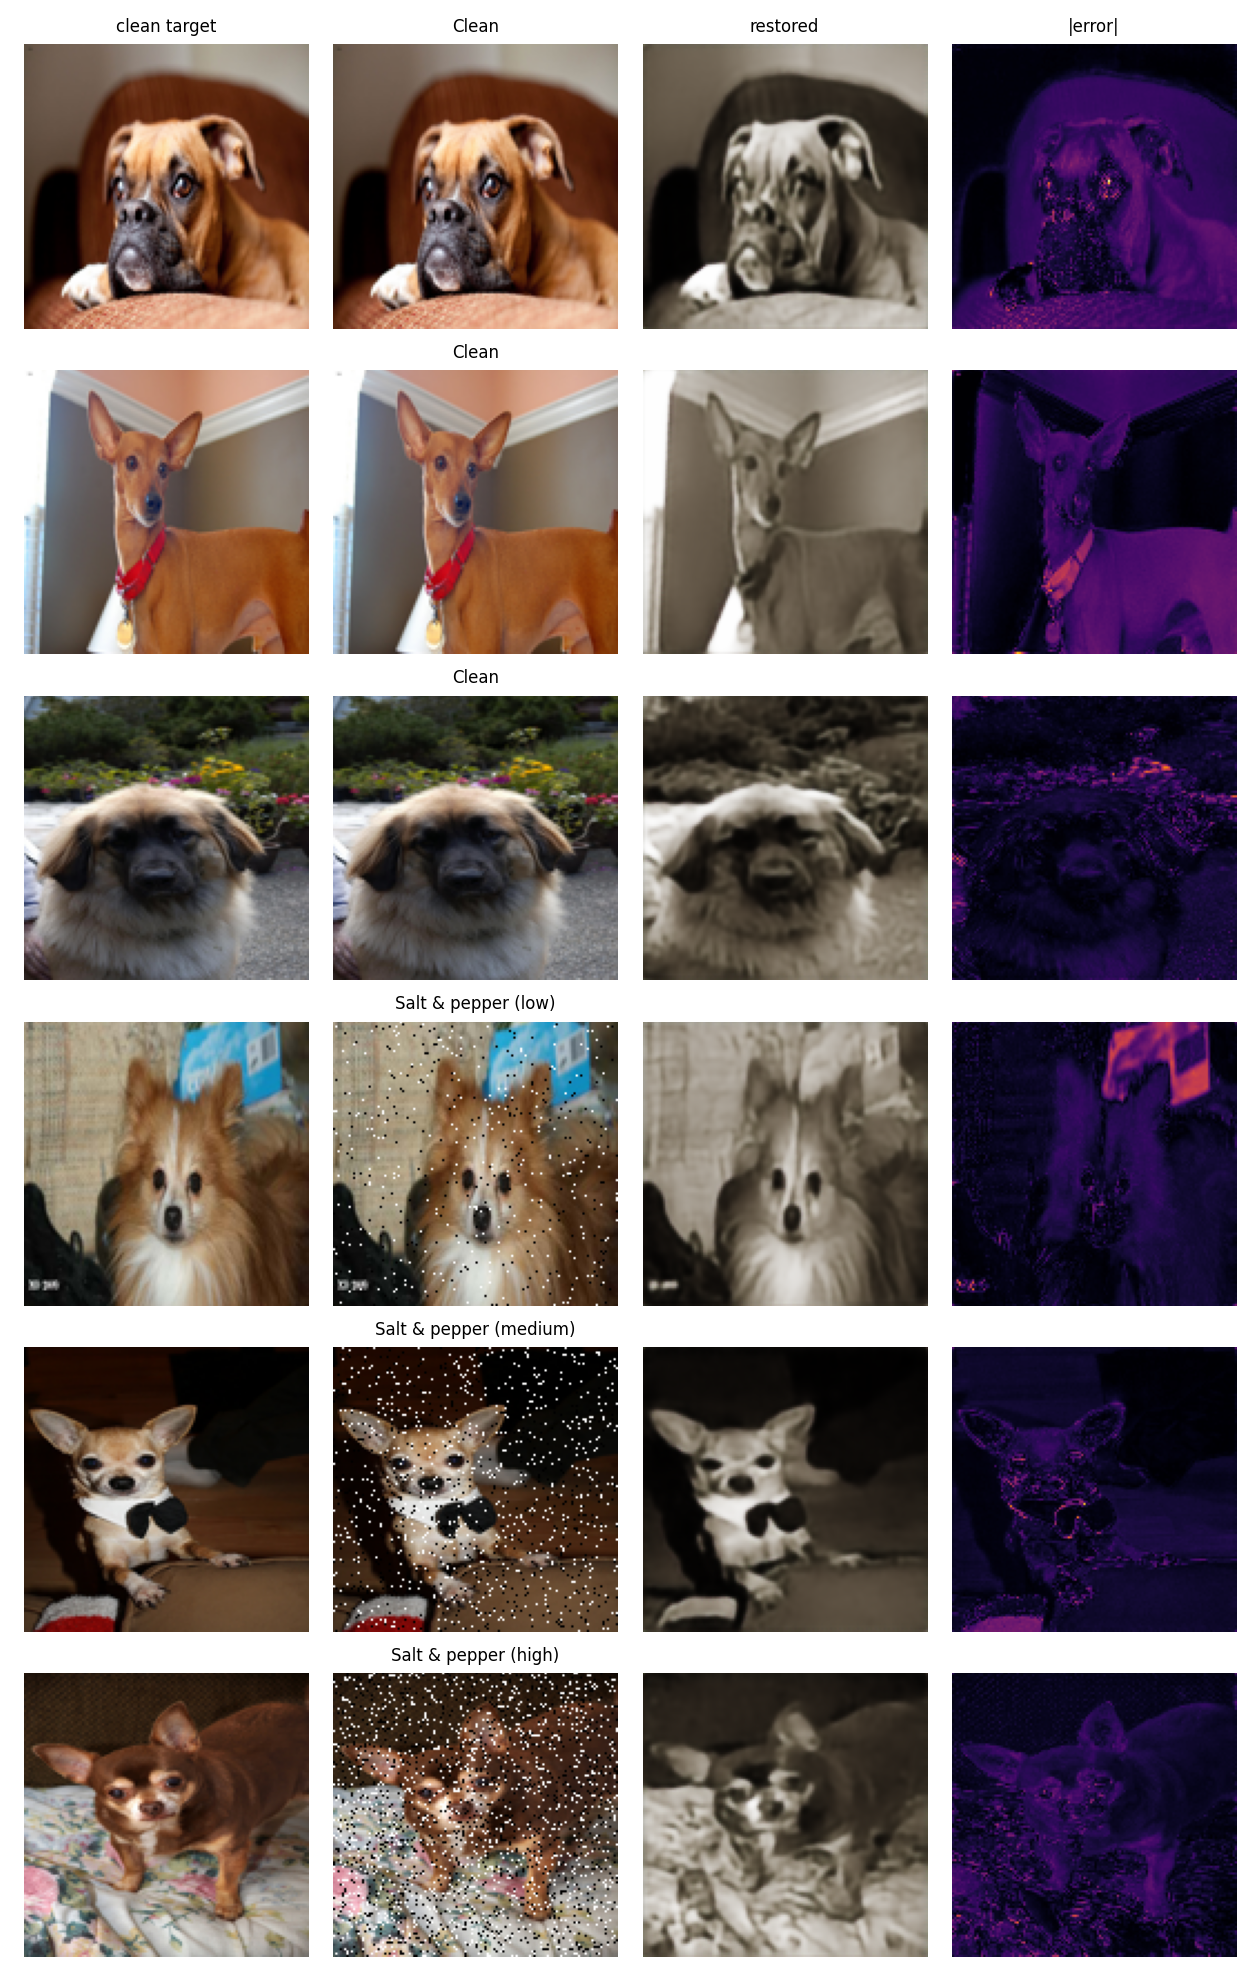
\includegraphics[width=\linewidth]{t1_examples_a_final.png}\caption{Task 1 examples (clean target, corrupted input, restored output, $|$error$|$). The second grid of six (twelve examples in total) is \texttt{t1\_examples\_b\_final.png} in the repository.}\label{fig:t1ex}\end{figure}}{}
\IfFileExists{figures/t1_failures_final.png}{\begin{figure}[t]\centering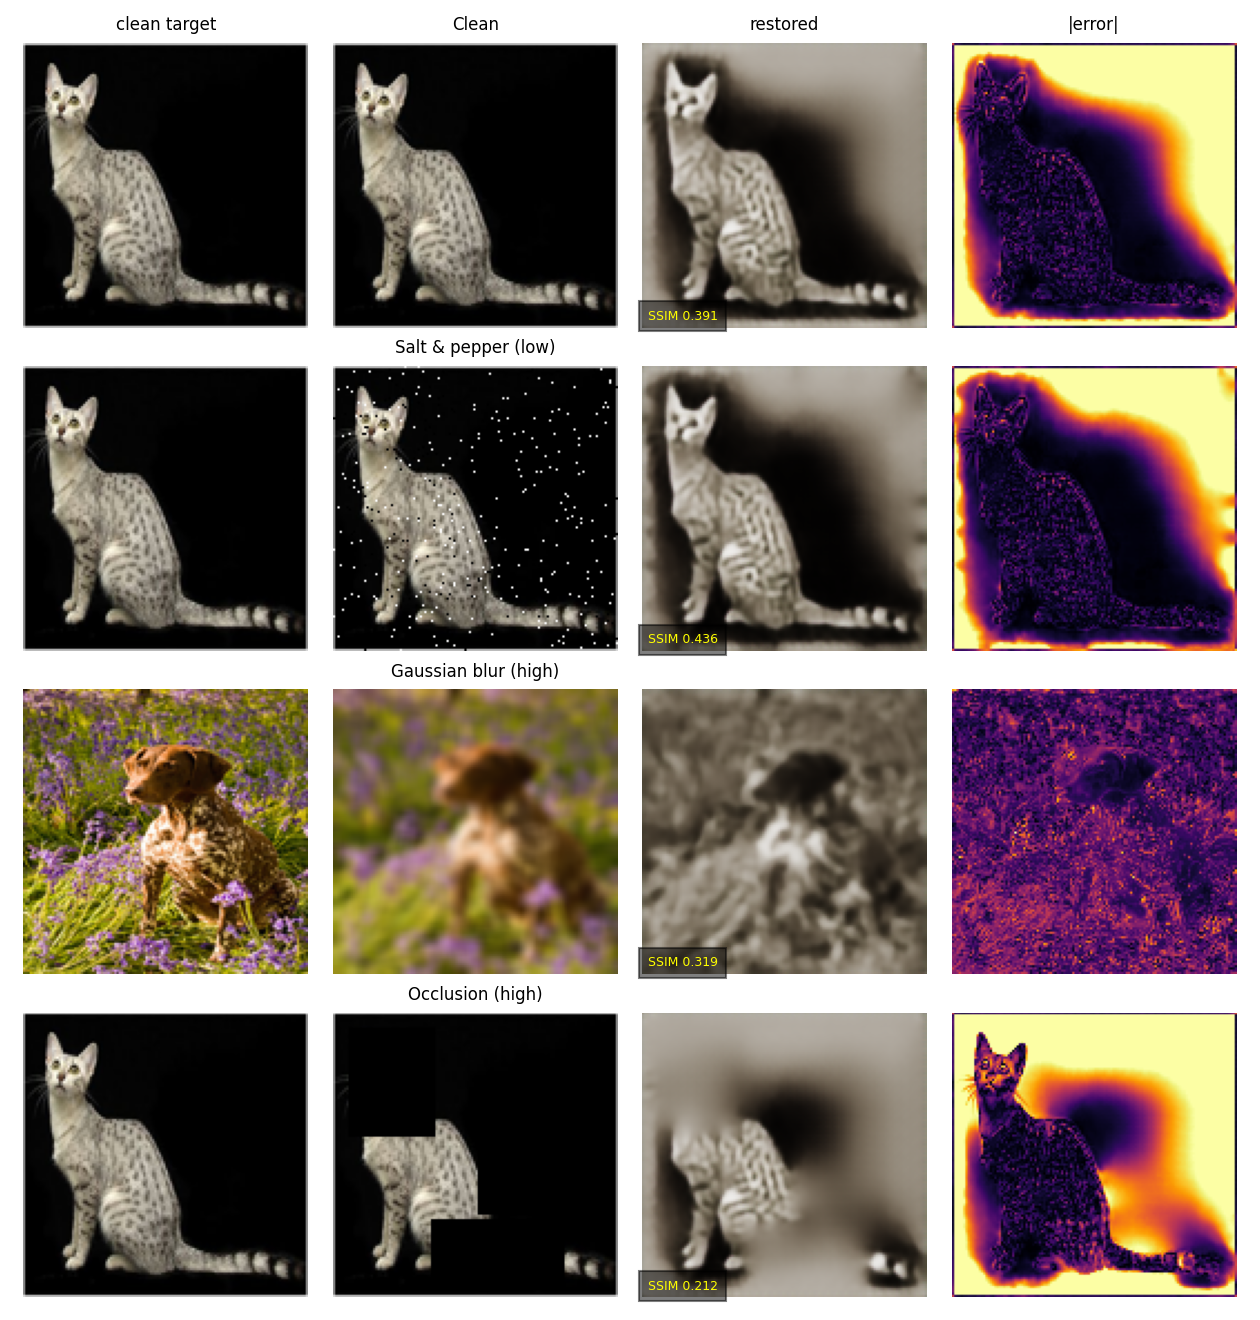
\includegraphics[width=\linewidth]{t1_failures_final.png}\caption{Task 1 failure cases (lowest SSIM per input condition).}\label{fig:t1fail}\end{figure}}{}
\IfFileExists{figures/t1_curves_final.png}{\begin{figure}[t]\centering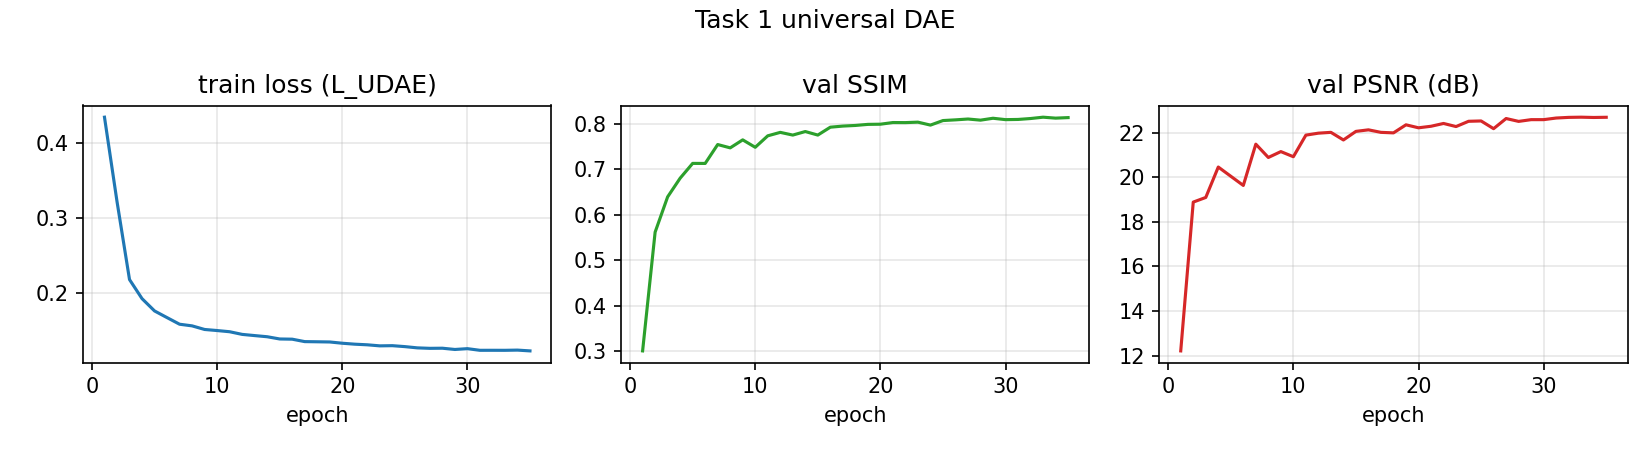
\includegraphics[width=\linewidth]{t1_curves_final.png}\caption{Task 1 training loss and validation SSIM/PSNR (35 epochs).}\label{fig:t1curve}\end{figure}}{}
\IfFileExists{figures/t1_optuna_history.png}{\begin{figure}[t]\centering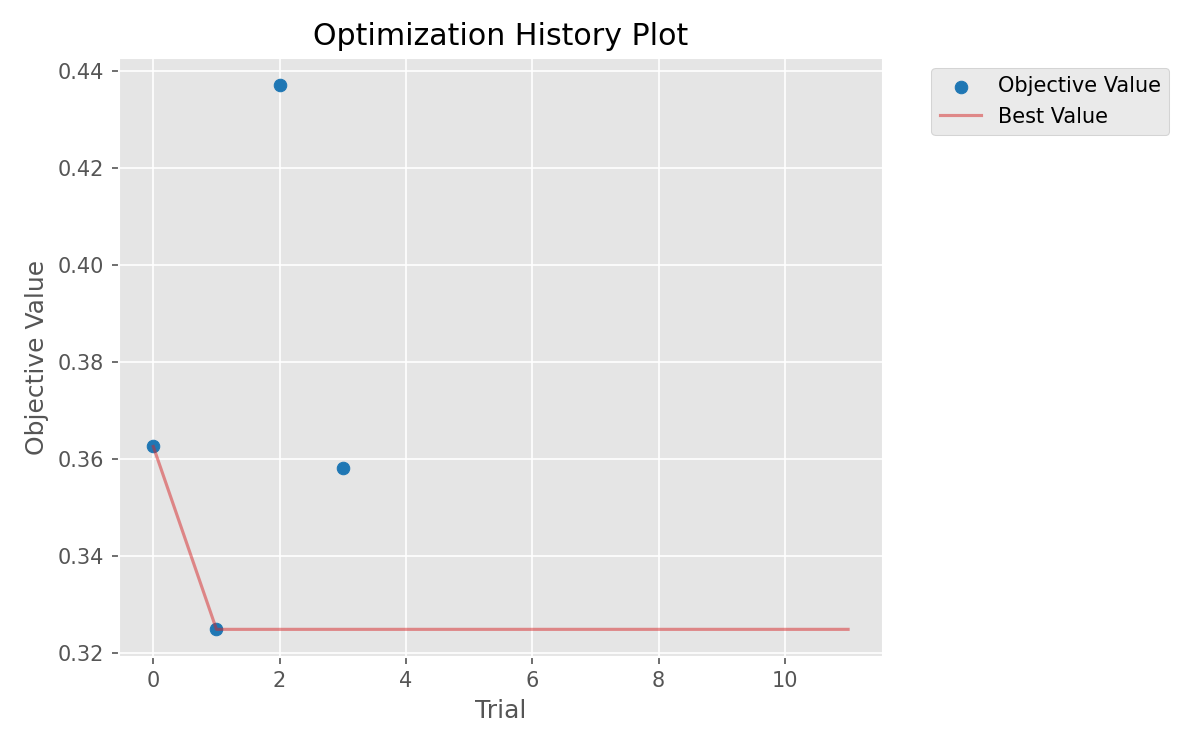
\includegraphics[width=0.9\linewidth]{t1_optuna_history.png}\caption{Task 1 Optuna optimisation history.}\label{fig:t1opt}\end{figure}}{}

\section{Task 2: Classifier and Hard-Routed Specialists}
A VGG-style CNN (four double-conv blocks, global average pooling, dropout, linear head) predicts \{clean, s\&p, blur, occlusion\}; cross-entropy is minimised on exactly class-balanced batches. Optuna (12 trials $\times$ 5 epochs, objective: validation macro-F1) tuned lr, batch, channel configuration (small/medium/wide), dropout and weight decay. Three specialists with the Task~1 architecture are trained only on their own corruption. To keep the search affordable we ran \emph{one shared} Optuna study (8 trials): each trial trains all three specialists for 4 epochs and is scored by the mean of their validation objectives; pruning acts on the running mean after each specialist. The selected configuration then trains three independent specialists for 25 epochs. At inference (Fig.~\ref{fig:t2arch}) the arg-max class selects one specialist, and clean inputs take an identity bypass.
\IfFileExists{figures/t2_hard.png}{\begin{figure}[t]\centering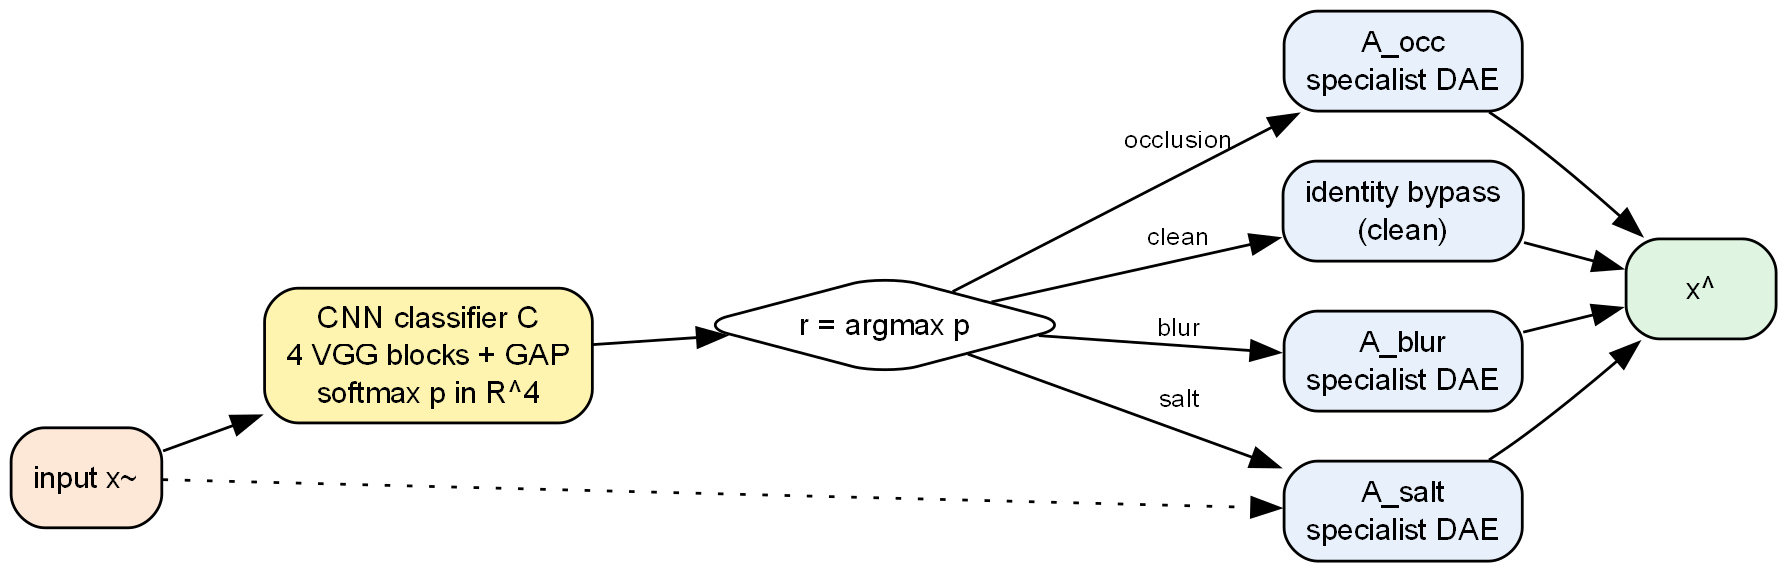
\includegraphics[width=\linewidth]{t2_hard.png}\caption{Hard routing.}\label{fig:t2arch}\end{figure}}{}
\textbf{Classifier.} The best Optuna trial (4 complete, 8 pruned) used the wide channel configuration (48--96--192--256), lr $5.4\cdot10^{-4}$, batch 64, dropout 0.39 and weight decay $6\cdot10^{-6}$ (validation macro-F1 0.988). On the test set it reaches 99.71\% accuracy and 0.995 macro-F1 (Table~\ref{tab:t2clf}, Fig.~\ref{fig:t2cm}). Salt-and-pepper is recognised perfectly; the remaining errors sit exactly at the expected class boundaries: 2.1\% of \emph{low}-severity occlusions (one 10\% rectangle) are called clean, typically when the black rectangle lands on an already dark background, and 0.7\% of clean images are called occlusion or blur (dark or out-of-focus photographs).
\textbf{Specialists.} The shared study (3 complete, 5 pruned) selected the same architecture as Task~1 (64 base channels, latent 32) with $\alpha=0.87$, i.e.\ the specialists prefer a larger pixel-wise L1 share than the universal model.
\textbf{Routing.} Table~\ref{tab:t2cmp} compares oracle and predicted routing. Because the classifier is so accurate, predicted routing loses only 0.02\,dB overall (27.46 vs.\ 27.48\,dB), and both are 5.3\,dB better than the universal DAE (Table~\ref{tab:cmp}). The identity bypass is the single largest gain: clean images stay at 50\,dB / 0.998 SSIM instead of 23\,dB. Of the 108 misrouted cases, the most harmful are \emph{clean$\rightarrow$occlusion} (15 cases, mean SSIM drop 0.32: an unnecessary inpainting pass blurs a perfect image) and \emph{clean$\rightarrow$blur} (9 cases, drop 0.10). Interestingly, the 76 \emph{occlusion$\rightarrow$clean} errors \emph{raise} SSIM on average (drop $-0.08$): a small black patch on a dark background costs less SSIM than the occlusion expert's global smoothing (Fig.~\ref{fig:t2mis}).
\begin{table}[t]\centering\caption{Corruption classifier on the test set (accuracy 99.71\%).}\label{tab:t2clf}
\begin{tabular}{lrrrr}\toprule
Class & Precision & Recall & F1 & Support\\ \midrule
Clean & 0.9777 & 0.9935 & 0.9855 & 3669 \\
S\&P & 1.0000 & 1.0000 & 1.0000 & 11007 \\
Blur & 0.9991 & 0.9994 & 0.9992 & 11007 \\
Occl. & 0.9986 & 0.9930 & 0.9958 & 11007 \\
Macro avg & 0.9939 & 0.9965 & 0.9951 & 36690 \\
\bottomrule\end{tabular}\end{table}
\begin{table}[t]\centering\caption{Hard routing: oracle vs.\ predicted routing (test).}\label{tab:t2cmp}\setlength{\tabcolsep}{3pt}
\begin{tabular}{lrrrrrr}\toprule
Input & PSNR$_{in}$ & PSNR$_{orc}$ & PSNR$_{pred}$ & SSIM$_{orc}$ & SSIM$_{pred}$ & Route\%\\ \midrule
Blur & 27.82 & 26.10 & 26.10 & 0.815 & 0.815 & 99.94 \\
Clean & 50.00 & 50.00 & 49.83 & 1.000 & 0.998 & 99.35 \\
Occl. & 13.57 & 22.12 & 22.11 & 0.737 & 0.738 & 99.30 \\
S\&P & 16.38 & 26.71 & 26.71 & 0.850 & 0.850 & 100.00 \\
Overall & 22.33 & 27.48 & 27.46 & 0.821 & 0.821 & 99.71 \\
\bottomrule\end{tabular}\end{table}
\IfFileExists{figures/t2_classifier_confusion.png}{\begin{figure}[t]\centering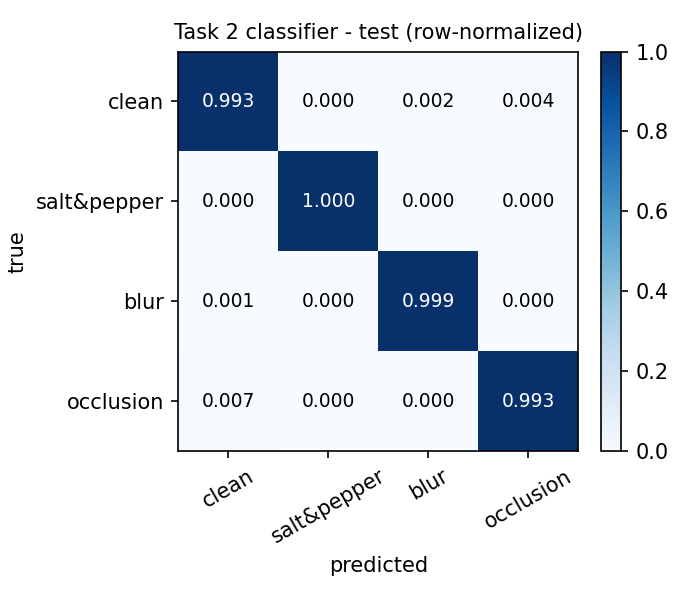
\includegraphics[width=0.8\linewidth]{t2_classifier_confusion.png}\caption{Row-normalised test confusion matrix of the classifier.}\label{fig:t2cm}\end{figure}}{}
\IfFileExists{figures/t2_hard_misrouted_failures.png}{\begin{figure}[t]\centering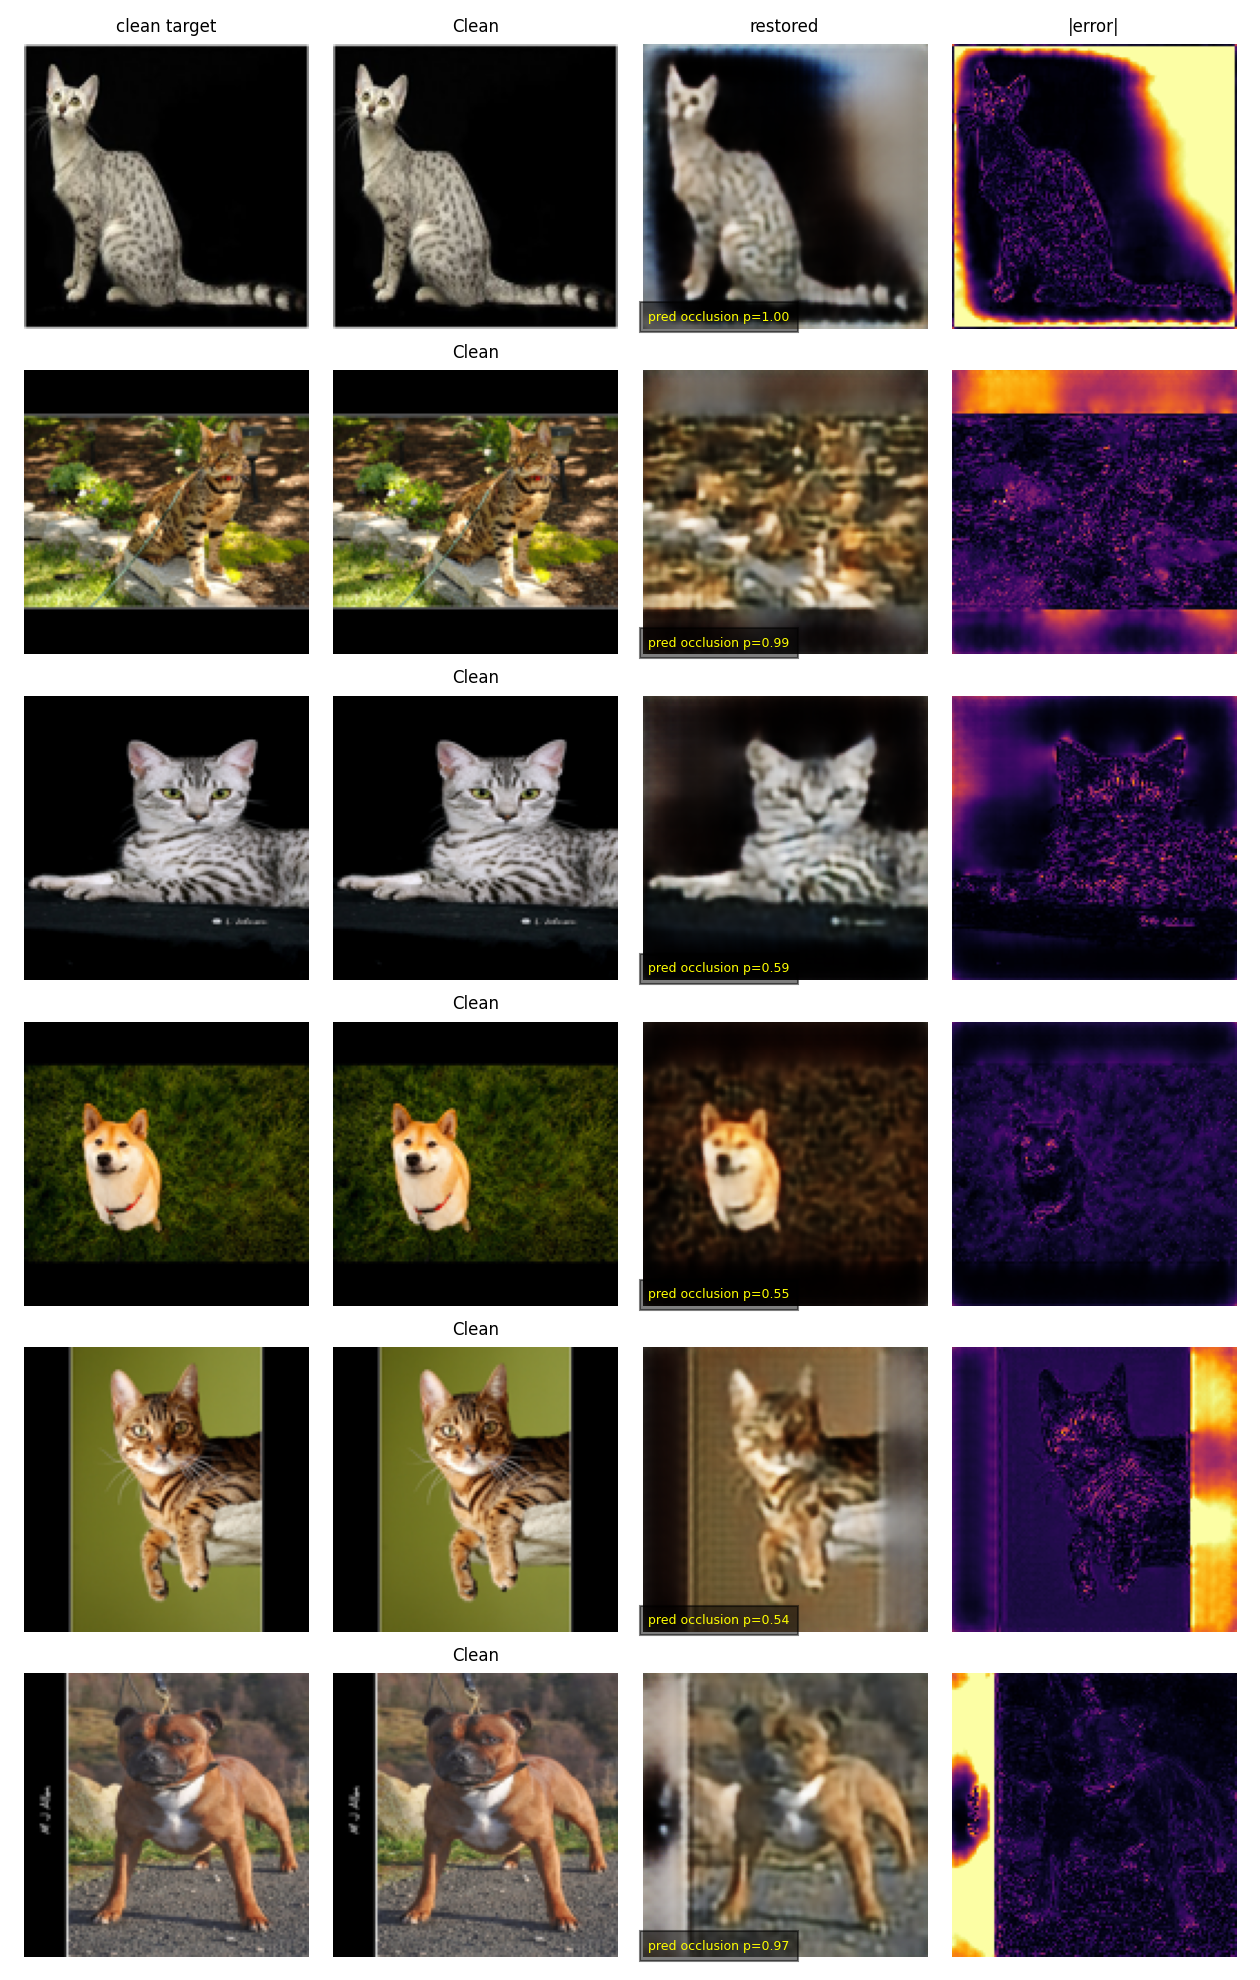
\includegraphics[width=\linewidth]{t2_hard_misrouted_failures.png}\caption{Misrouted test cases with the largest SSIM drop relative to oracle routing.}\label{fig:t2mis}\end{figure}}{}

\section{Task 3: Jointly Trained Soft Mixture-of-Experts}
The gate $G$ shares the classifier architecture and weights; the experts are the three specialists plus an identity branch (Fig.~\ref{fig:t3arch}): $w=\mathrm{softmax}(G(\tilde x)/\tau)$, $\hat x=w_0\tilde x+\sum_{k=1}^3 w_kA_k(\tilde x)$. Training: (1) warm-up with experts frozen, only $G$ trained (lr $10^{-3}$); (2) joint fine-tuning of all parameters with a smaller learning rate. Specialist BatchNorm statistics are kept frozen during fine-tuning, a standard precaution when fine-tuning pretrained networks on a shifted input mixture. The loss is $\lambda_1\mathcal L_1+\lambda_s(1-\mathrm{SSIM})+\lambda_c\mathcal L_{CE}+\lambda_b\sum_k(\bar w_k-\frac14)^2$, where $\bar w_k$ is the batch-mean weight. Because our batches are exactly class-balanced, a uniform \emph{average} routing is the correct target, while individual images can still be routed sharply (a property that per-sample entropy penalties would destroy); this mirrors the load-balancing losses of~\cite{shazeer2017,fedus2022}. Optuna (6 trials, 1 warm-up + 3 joint epochs) tuned the joint lr, $\tau\in[0.5,2]$, $\lambda_c$, $\lambda_b$ and $\lambda_1$ (with $\lambda_s=1-\lambda_1$). Trials were pruned on median performance \emph{or} routing collapse (any branch with mean validation weight $<2\%$).
\IfFileExists{figures/t3_moe.png}{\begin{figure}[t]\centering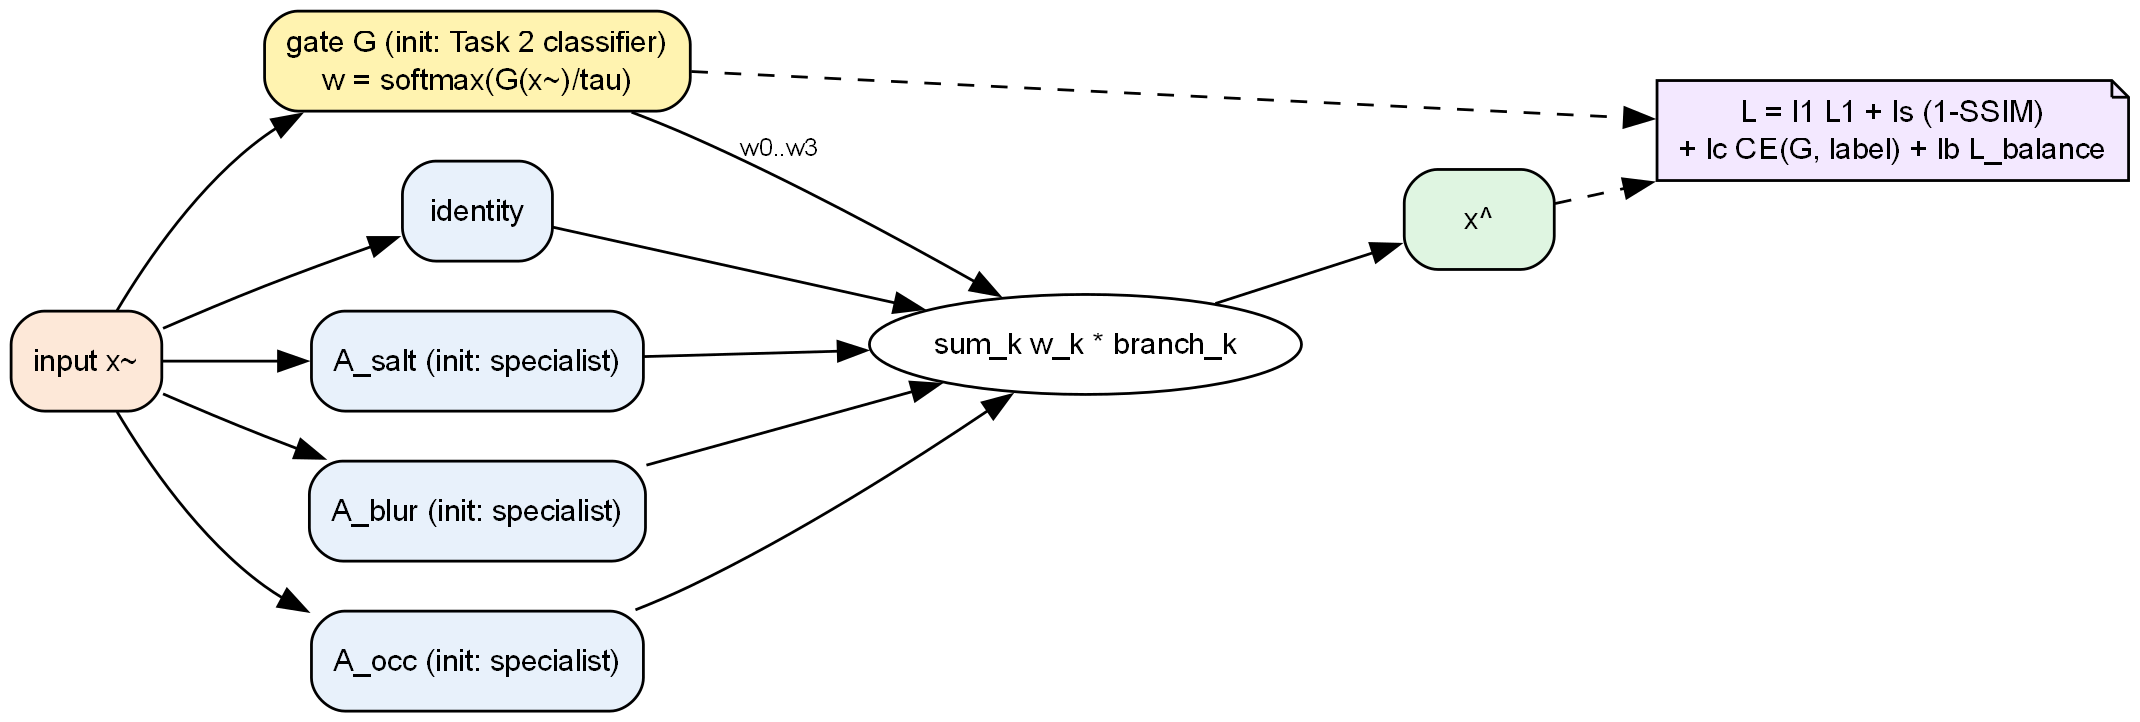
\includegraphics[width=\linewidth]{t3_moe.png}\caption{Soft MoE with identity branch.}\label{fig:t3arch}\end{figure}}{}
\textbf{Optuna.} Of 6 trials, 2 were pruned; none for routing collapse, showing that the balance and cross-entropy terms together prevent collapse. The best configuration used joint lr $3.6\cdot10^{-5}$, $\tau=1.93$, $\lambda_c=0.175$, $\lambda_b=0.016$ and $\lambda_1=0.57$ (validation SSIM 0.866). A high temperature was preferred, which keeps gradients flowing to non-selected experts during joint training.
\textbf{Reconstruction.} The soft MoE has the best overall SSIM (0.832 vs.\ 0.821 hard and 0.792 universal, Table~\ref{tab:cmp}) and matches hard routing in PSNR (27.48\,dB), with gains on salt-and-pepper (26.90 vs.\ 26.71\,dB) and blur (26.43 vs.\ 26.10\,dB) that come from jointly fine-tuning the experts through the mixture. Clean images are reproduced at 48.7\,dB / 0.998 SSIM through the identity branch (Table~\ref{tab:t3}).
\textbf{Routing behaviour.} Table~\ref{tab:t3w} and Fig.~\ref{fig:t3heat} show a nearly diagonal routing: salt-and-pepper images give 0.96--0.98 weight to the salt-and-pepper expert, blur 0.91--0.93 to the blur expert, and medium/high occlusion $\geq0.99$ to the occlusion expert. The interesting case is \emph{low} occlusion, where 23\% of the weight goes to the identity branch and 75\% to the occlusion expert, a genuine soft blend: the gate has learned that inpainting one small rectangle should not smooth the other 90\% of the image. Blurred inputs similarly keep about 7\% identity weight. No branch is inactive (mean test weights 0.14/0.29/0.28/0.28; the identity mean is lower simply because only 10\% of test cases are clean), and off-target weight is at most 8.8\% for any true class, so no expert dominates unrelated inputs. 88\% of images are routed with $w_{\max}>0.9$ and only 1.6\% are distributed ($w_{\max}<0.6$); Fig.~\ref{fig:t3dist} shows the most distributed examples.
\textbf{Two simultaneous corruptions.} On 500 test images corrupted with blur ($k{=}5,\sigma{=}1.5$) \emph{and} salt-and-pepper ($p{=}0.08$), the hard router sends all 500 to the salt-and-pepper expert and the MoE also puts 0.99 weight on it (24.74 vs.\ 24.61\,dB). This is an honest negative result: trained with single-label cross-entropy, the gate is confident even on out-of-distribution mixtures and does not spread weight. Training on mixed corruptions with soft multi-label targets would be the natural fix.
\begin{table}[t]\centering\caption{Task 3 soft MoE on the test set.}\label{tab:t3}\setlength{\tabcolsep}{4pt}
\begin{tabular}{llrrrr}\toprule
Input & Sev. & PSNR$_{in}$ & PSNR$_{out}$ & SSIM$_{in}$ & SSIM$_{out}$\\ \midrule
Clean & none & 50.00 & 48.69 & 1.000 & 0.998 \\
S\&P & low & 20.13 & 27.11 & 0.602 & 0.867 \\
S\&P & medium & 15.87 & 26.92 & 0.340 & 0.861 \\
S\&P & high & 13.14 & 26.67 & 0.204 & 0.850 \\
Blur & low & 32.34 & 27.28 & 0.944 & 0.870 \\
Blur & medium & 26.77 & 27.09 & 0.806 & 0.854 \\
Blur & high & 24.35 & 24.93 & 0.692 & 0.748 \\
Occl. & low & 16.70 & 23.68 & 0.862 & 0.843 \\
Occl. & medium & 13.27 & 22.18 & 0.726 & 0.754 \\
Occl. & high & 10.75 & 20.24 & 0.536 & 0.677 \\
\bottomrule\end{tabular}\end{table}
\begin{table}[t]\centering\caption{Mean soft-MoE routing weights per true corruption and severity (test).}\label{tab:t3w}\setlength{\tabcolsep}{4pt}
\begin{tabular}{llrrrr}\toprule
Input & Sev. & $w_{id}$ & $w_{s\&p}$ & $w_{blur}$ & $w_{occ}$\\ \midrule
Clean & none & 0.941 & 0.002 & 0.030 & 0.028 \\
S\&P & low & 0.020 & 0.965 & 0.009 & 0.007 \\
S\&P & medium & 0.011 & 0.981 & 0.005 & 0.003 \\
S\&P & high & 0.013 & 0.977 & 0.006 & 0.004 \\
Blur & low & 0.077 & 0.002 & 0.913 & 0.008 \\
Blur & medium & 0.065 & 0.002 & 0.926 & 0.007 \\
Blur & high & 0.069 & 0.002 & 0.922 & 0.008 \\
Occl. & low & 0.227 & 0.012 & 0.010 & 0.751 \\
Occl. & medium & 0.007 & 0.006 & 0.001 & 0.986 \\
Occl. & high & 0.000 & 0.002 & 0.000 & 0.998 \\
\bottomrule\end{tabular}\end{table}
\IfFileExists{figures/t3_moe_routing_heatmap.png}{\begin{figure}[t]\centering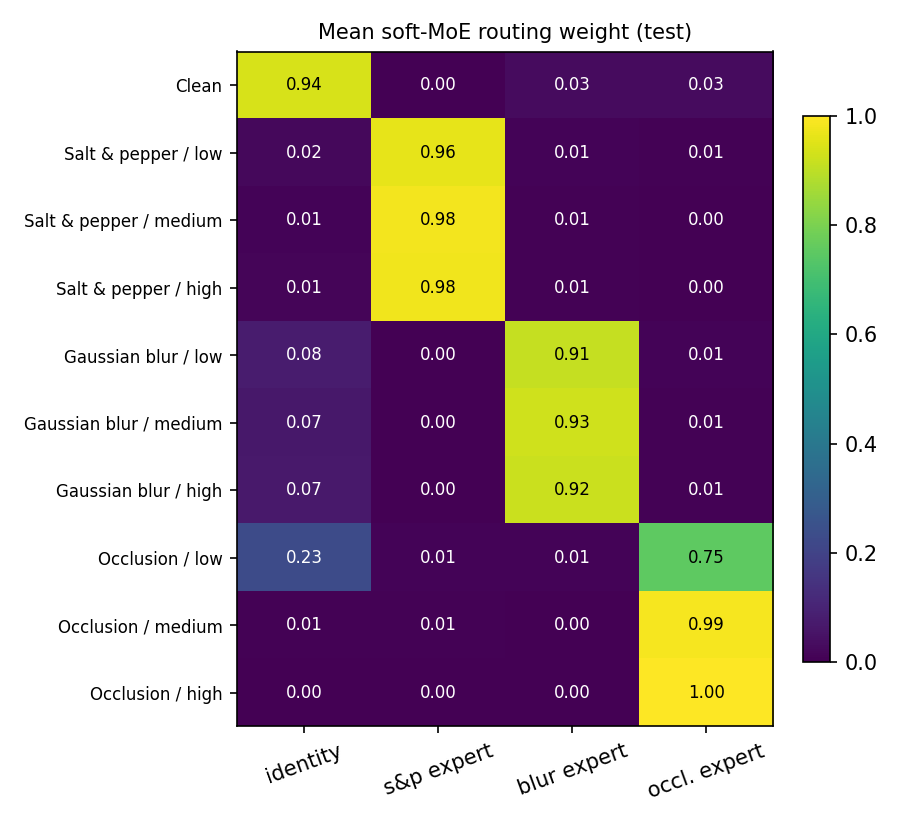
\includegraphics[width=0.85\linewidth]{t3_moe_routing_heatmap.png}\caption{Routing heatmap: mean branch weight for every true corruption and severity (test).}\label{fig:t3heat}\end{figure}}{}
\IfFileExists{figures/t3_moe_examples_distributed.png}{\begin{figure}[t]\centering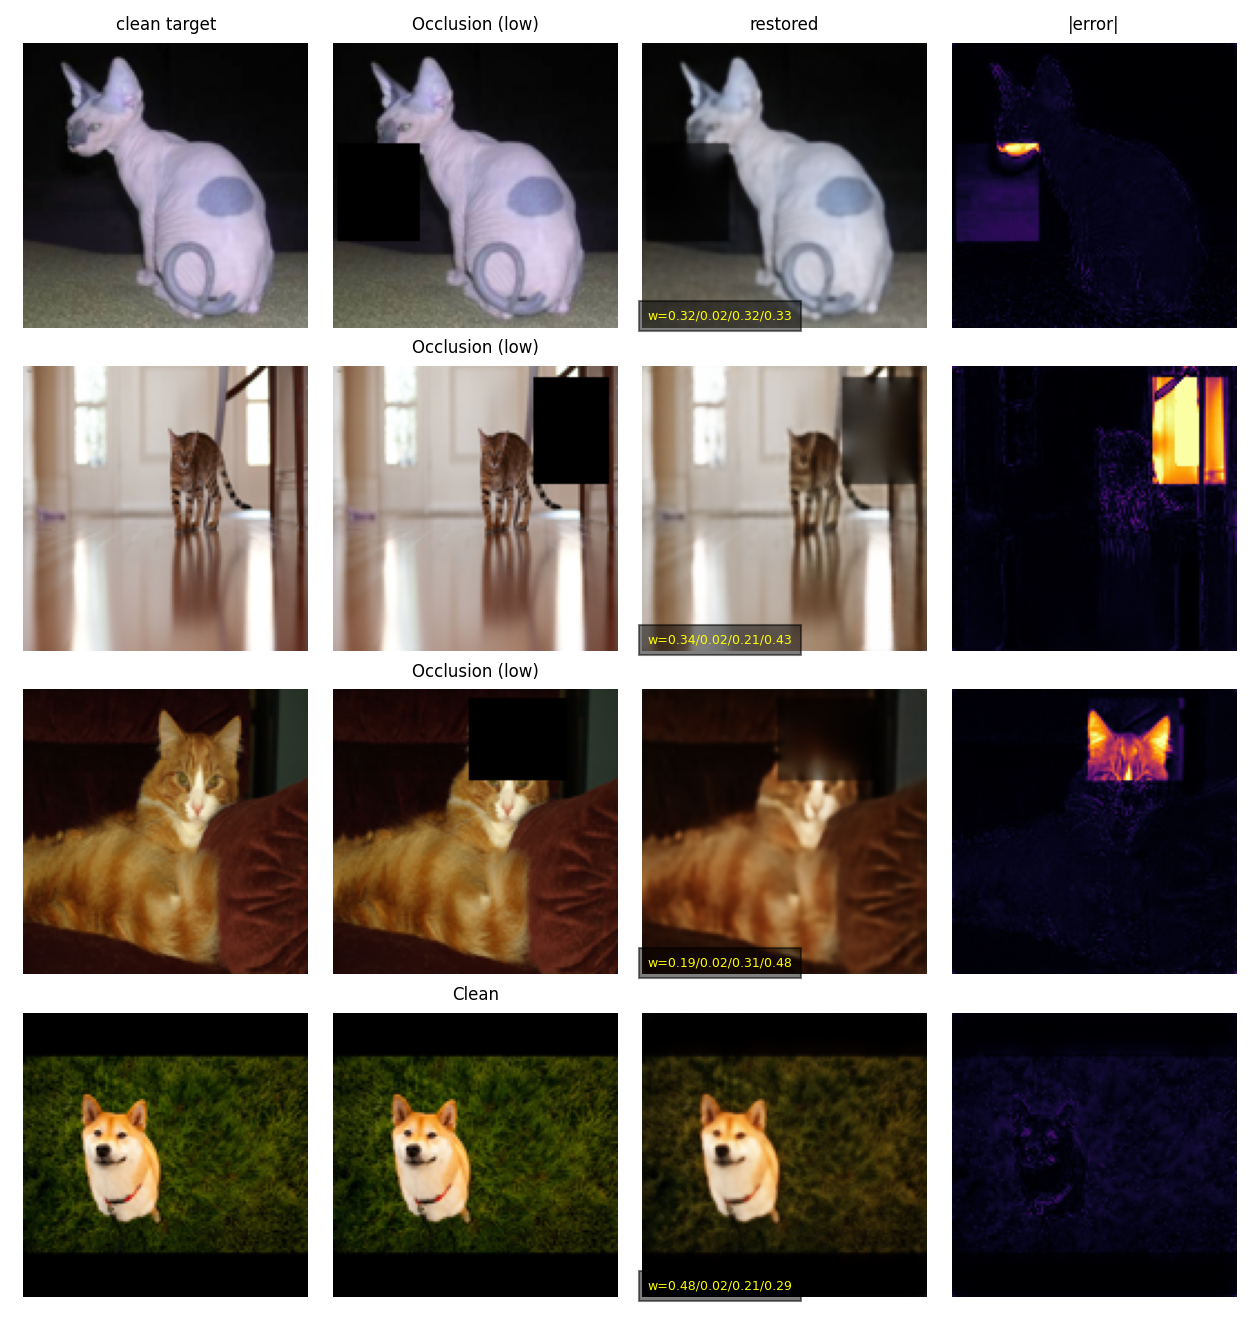
\includegraphics[width=\linewidth]{t3_moe_examples_distributed.png}\caption{Images with the most distributed routing (weights printed as identity/s\&p/blur/occlusion).}\label{fig:t3dist}\end{figure}}{}
\IfFileExists{figures/t3_moe_curves.png}{\begin{figure}[t]\centering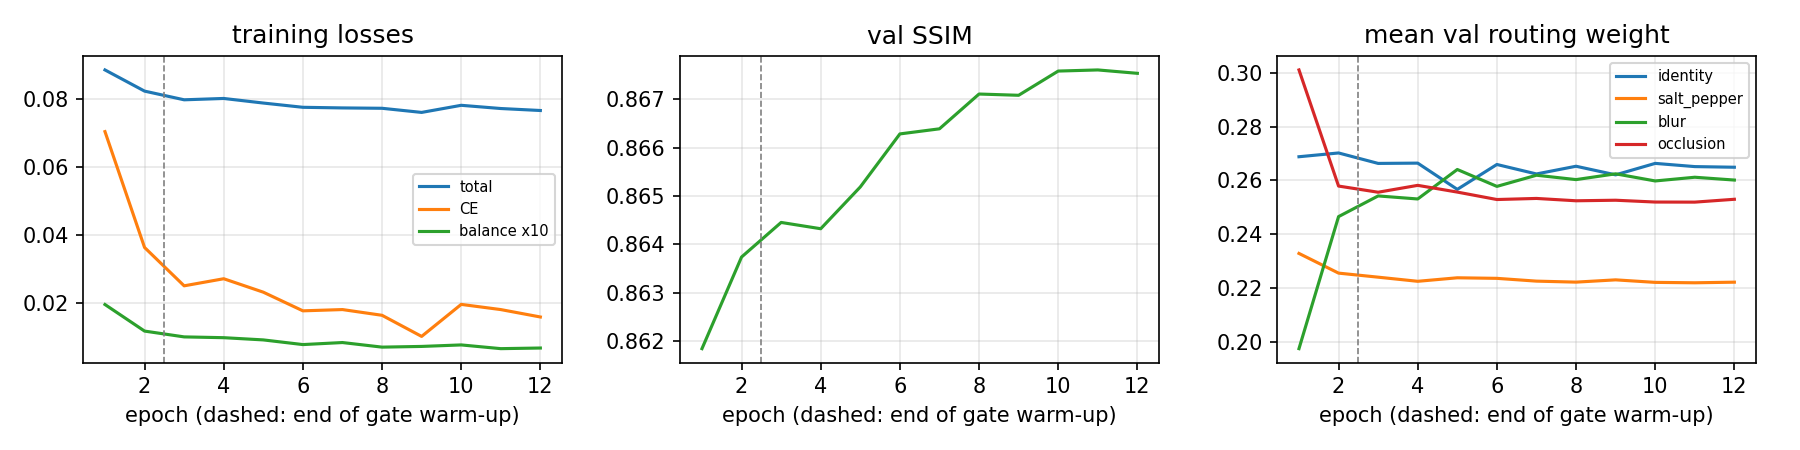
\includegraphics[width=\linewidth]{t3_moe_curves.png}\caption{MoE training: losses, validation SSIM and mean routing weights (dashed line: end of gate warm-up).}\label{fig:t3curve}\end{figure}}{}

\section{Task 4: Style-Conditioned Face-to-Sketch cGAN}
FS2K's official train/test definitions are used; 15\% of the training portion (stratified by style, seed 42) forms the validation set, and the test set is never used for training or model selection. Photos (RGB) and sketches (grayscale) are resized to $128\times128$ and kept paired by name. Augmentation (random horizontal flip and an 8-pixel reflect-pad random crop) is drawn \emph{once} per pair and applied identically to photo and sketch, preserving pixel correspondence.
The generator (Fig.~\ref{fig:t4arch}) is a U-Net (6 down-sampling blocks to $2\times2$, 5 up-sampling blocks with skips, dropout in the first three decoder blocks, tanh output). A learned \texttt{nn.Embedding}(3,$E$) conditions both networks: in $G$ it is tiled and concatenated to the photo and also projected and added at the bottleneck; in the PatchGAN $D$ ($14\times14$ logits for $128^2$ inputs) it is tiled and concatenated to the photo--sketch pair. Losses: $\mathcal L_D=\frac12[\mathrm{BCE}(D(x,y,s),1)+\mathrm{BCE}(D(x,G(x,s),s),0)]$, $\mathcal L_G=\mathrm{BCE}(D(x,G(x,s),s),1)+\lambda_{L1}\|y-G(x,s)\|_1$; Adam$(0.5,0.999)$ with the pix2pix schedule (constant, then linear decay). The D-real, D-fake, G-adversarial and G-L1 losses and validation SSIM/L1 are logged separately, and the same 8 validation photos are rendered every 5 epochs. Optuna (8-epoch trials) tuned both learning rates, batch, base channels, dropout, embedding size and $\lambda_{L1}\in[10,200]$; the selected configuration was retrained for the full schedule. Because pixel metrics favour blurry outputs, the \emph{final} generator (end of LR decay) is deployed, not the epoch with the best validation SSIM.
\IfFileExists{figures/t4_cgan.png}{\begin{figure}[t]\centering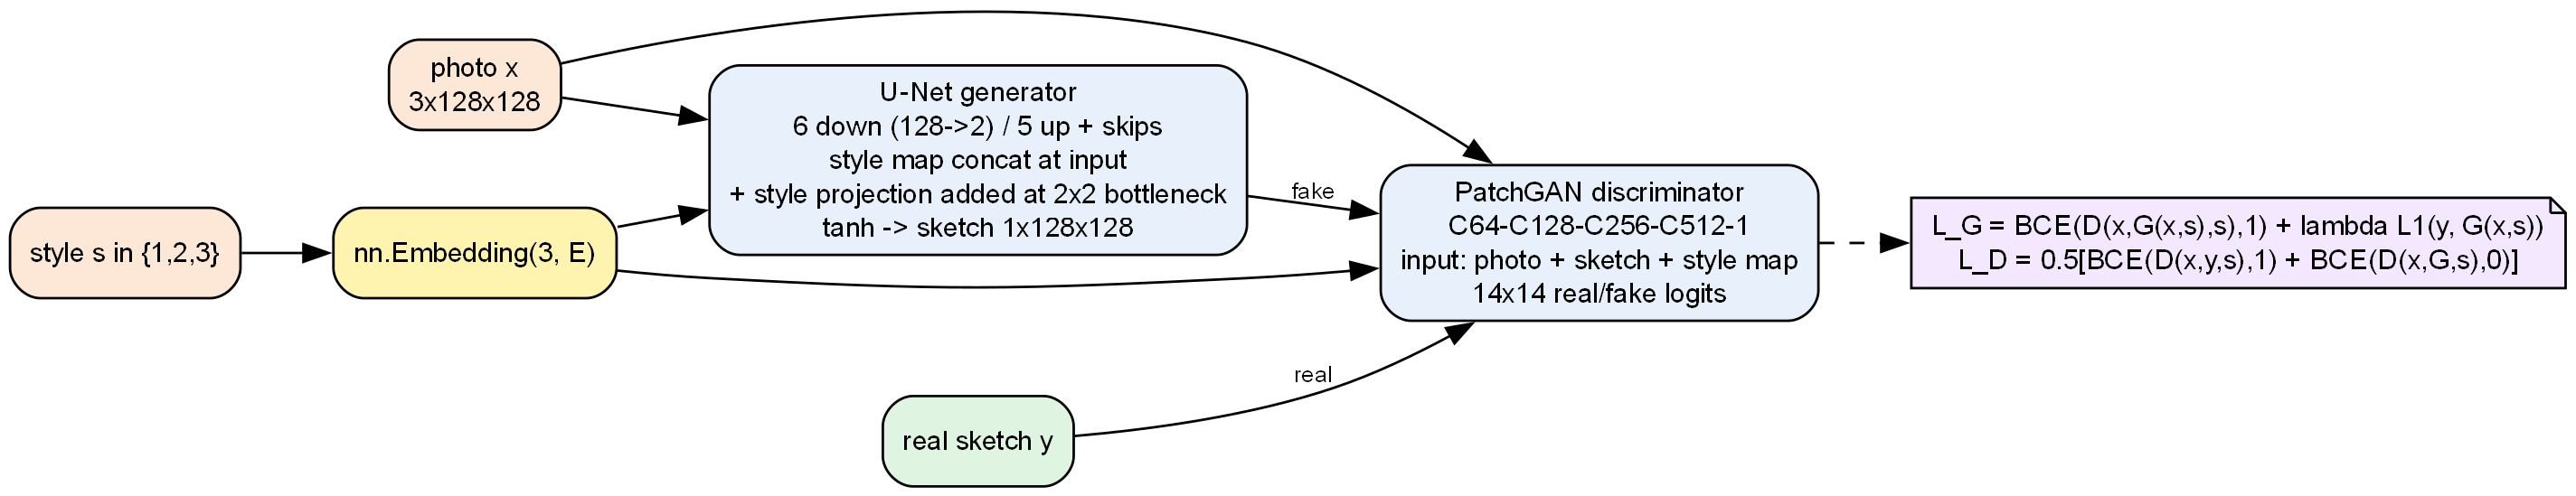
\includegraphics[width=\linewidth]{t4_cgan.png}\caption{Style-conditioned cGAN.}\label{fig:t4arch}\end{figure}}{}
\textbf{Optuna.} Four 8-epoch trials were run (3 complete, 1 pruned; the budget was reduced after two Colab disconnections). The best configuration used $\mathrm{lr}_G=1.2\cdot10^{-4}$, $\mathrm{lr}_D=4.3\cdot10^{-4}$, batch 4, 64 base channels, dropout 0.30, a 32-dimensional style embedding and $\lambda_{L1}=121$ (validation SSIM 0.477). Optuna kept $\lambda_{L1}$ close to the pix2pix value of 100 but preferred a discriminator learning rate $3.6\times$ larger than the generator's, which compensated for the weak early discriminator signal of the small-batch regime. The configuration was retrained for 40 epochs.
\textbf{Training dynamics.} Fig.~\ref{fig:t4curve} shows the separately logged losses. The discriminator's real and fake losses fall from 0.76/0.75 to 0.16/0.15 while the generator's adversarial loss rises from 0.78 to 2.64: towards the end the discriminator increasingly wins, but the L1 term keeps the generator anchored (train L1 0.29$\rightarrow$0.21, validation L1 0.113$\rightarrow$0.104). Validation SSIM peaked at epoch 22 (0.477) and ended at 0.452. Following pix2pix practice we deploy the final generator, because later epochs produce crisper strokes even when pixel SSIM is slightly lower.
\textbf{Results.} Table~\ref{tab:t4} reports test metrics per style. FS2K's official test split is strongly unbalanced (619 / 381 / 46 images for styles 1/2/3), whereas our training split is nearly balanced (303 / 298 / 298), so we report every style separately. Style~3 (soft shading) is reproduced best (SSIM 0.582, PSNR 18.3\,dB) and Style~2 (dense pencil hatching) worst (0.348, 11.8\,dB): hatching patterns are stochastic, and a pixel-wise metric penalises any plausible but differently placed stroke. The style-control grid (Fig.~\ref{fig:t4style}) shows that the learned embedding genuinely controls the output: the same photograph is rendered with light contours (Style~1), heavy dark hatching (Style~2) or soft grey shading (Style~3), while identity, glasses, hats and hairstyles are preserved. This confirms that the condition is used by the network and is not just an interface label.
\textbf{Failure cases.} The six lowest-SSIM test cases (Fig.~\ref{fig:t4fail}) are all Style~1/2 portraits of people with long, light-coloured hair. They share a repeated inverted-V ``nose'' stroke that ignores the actual nose, a template-like artefact typical of mild mode collapse in conditional GANs trained on small datasets (fewer than 900 training pairs). Long hair is also drawn as dense vertical strokes rather than the artist's flowing contours. More data, a perceptual (VGG) loss or feature matching, and spectral normalisation in $D$ would be the next steps.
\begin{table}[t]\centering\caption{Task 4 test results per sketch style (FS2K official test split).}\label{tab:t4}
\begin{tabular}{lrrrr}\toprule
Style & $n$ & L1 & SSIM & PSNR (dB)\\ \midrule
Style 1 & 619 & 0.087 & 0.472 & 16.66 \\
Style 2 & 381 & 0.165 & 0.348 & 11.80 \\
Style 3 & 46 & 0.068 & 0.582 & 18.31 \\
Overall & 1046 & 0.114 & 0.432 & 14.96 \\
\bottomrule\end{tabular}\end{table}
\IfFileExists{figures/t4_cgan_style_control.png}{\begin{figure}[t]\centering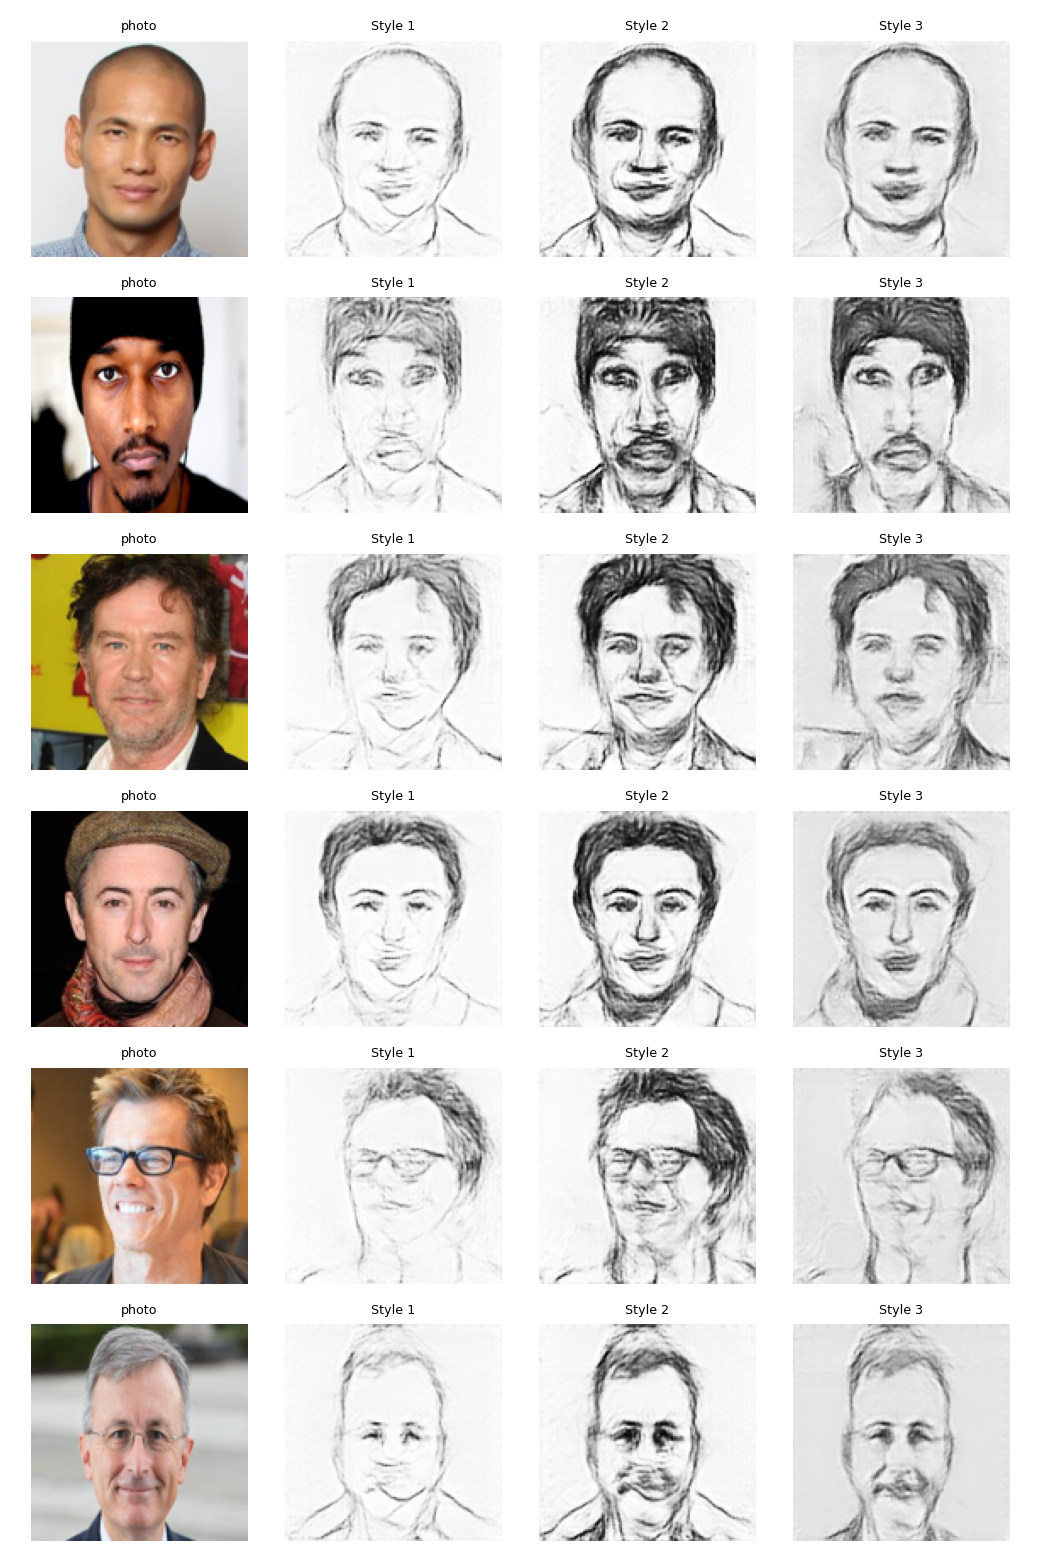
\includegraphics[width=\linewidth]{t4_cgan_style_control.png}\caption{Style control: each test photograph rendered with all three style conditions.}\label{fig:t4style}\end{figure}}{}
\IfFileExists{figures/t4_cgan_curves.png}{\begin{figure}[t]\centering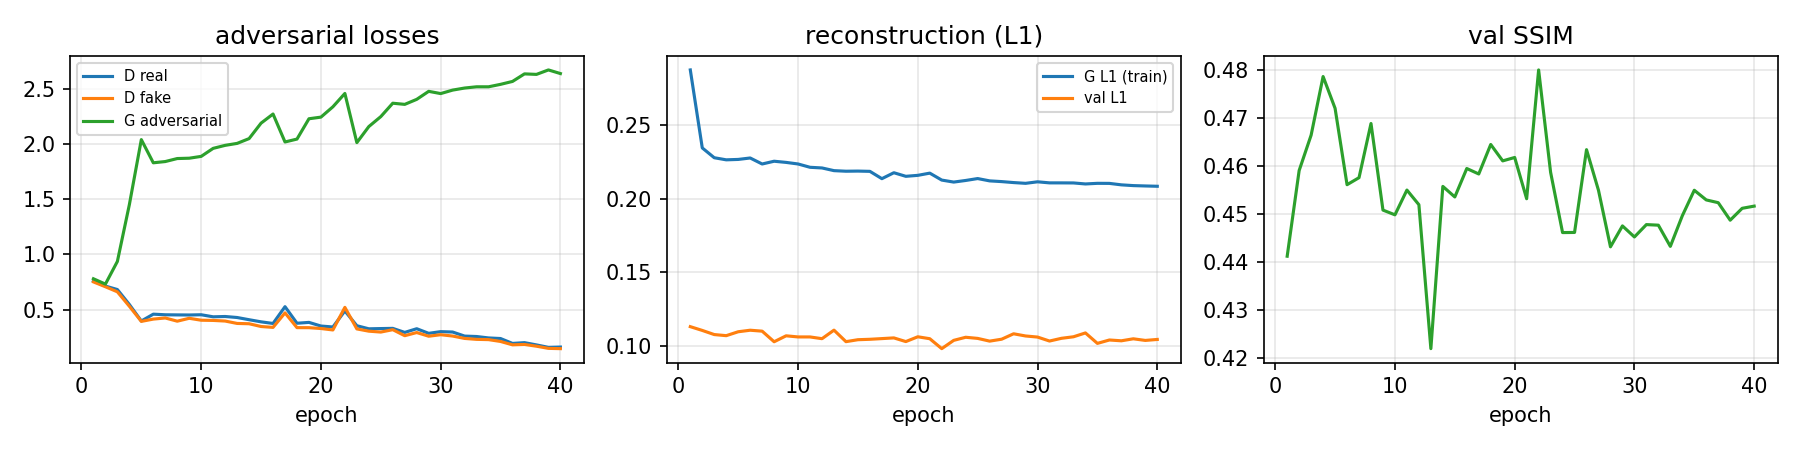
\includegraphics[width=\linewidth]{t4_cgan_curves.png}\caption{Task 4 training: discriminator real/fake loss, generator adversarial loss, train/validation L1 and validation SSIM.}\label{fig:t4curve}\end{figure}}{}
\IfFileExists{figures/t4_cgan_failures.png}{\begin{figure}[t]\centering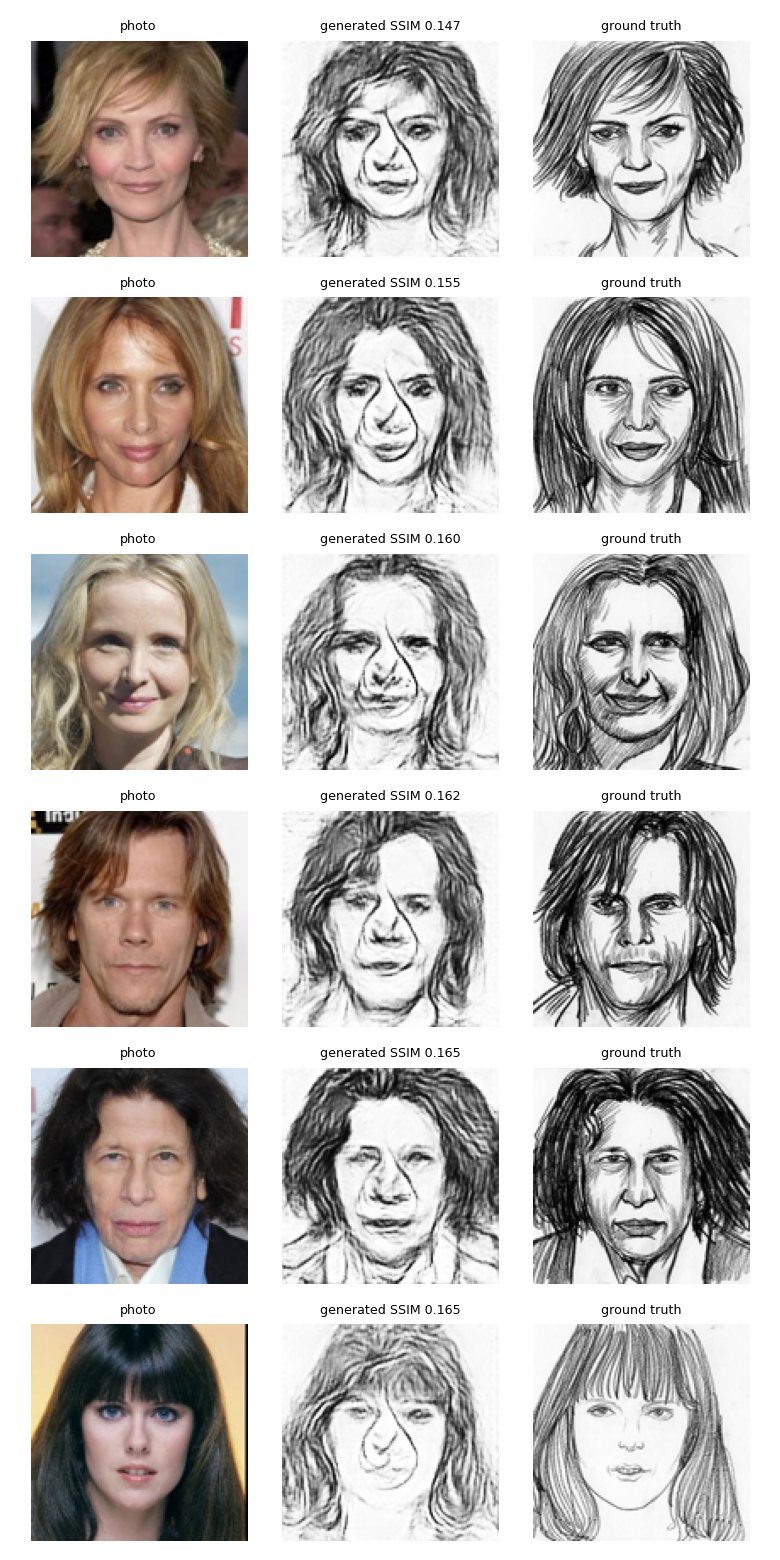
\includegraphics[width=0.62\linewidth]{t4_cgan_failures.png}\caption{Task 4 failure cases (lowest test SSIM): photo, generated sketch, ground truth.}\label{fig:t4fail}\end{figure}}{}
\IfFileExists{figures/t4_cgan_test_examples.png}{\begin{figure}[t]\centering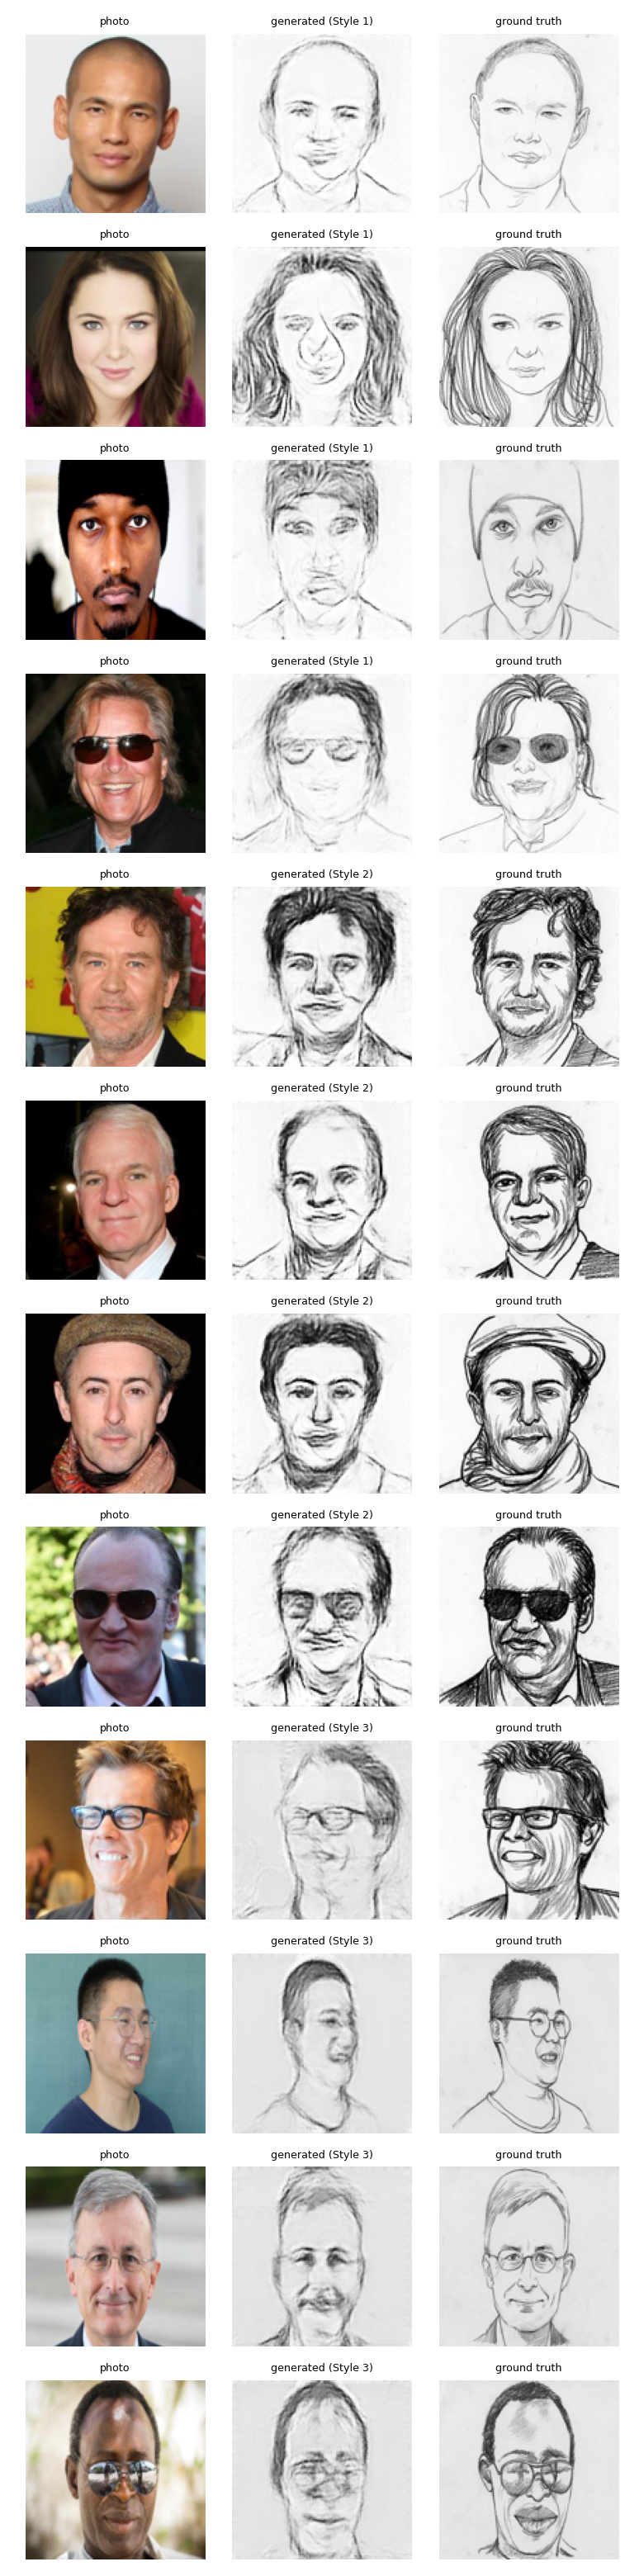
\includegraphics[height=0.85\textheight]{t4_cgan_test_examples.png}\caption{Task 4 test examples, four per style: photo, generated sketch (true style), ground truth.}\label{fig:t4ex}\end{figure}}{}

\section{Application Design and Deployment}
The interface was first designed in Google Stitch and implemented in React + Tailwind CSS (Figs.~\ref{fig:appshots} and~\ref{fig:appsketch}): a sidebar with the four required workspaces (Universal Restoration, Hard-Routed Restoration, Soft Mixture-of-Experts Restoration, Face-to-Sketch Generator) and a System page. Each restoration workspace lets the user upload an image or pick a sample, optionally apply a runtime corruption with test-set severities and a seed, and shows the clean reference, model input, output and error map together with PSNR/L1, inference time per stage, classifier probabilities with the selected expert, or the four MoE weights as bars and a stacked contribution strip. The sketch workspace supports upload or webcam capture, three styles, side-by-side display and download. The FastAPI backend validates type and size (415/413/422 errors), decodes with EXIF correction, resizes exactly as in training, runs ONNX Runtime and returns base64 PNGs plus JSON metadata (Fig.~\ref{fig:apparch}). It exposes \texttt{/api/health}, \texttt{/api/info}, \texttt{/api/restore/\{universal,hard,soft\}}, \texttt{/api/sketch} and \texttt{/api/corrupt}. Frontend (nginx) and backend run in separate containers; \texttt{docker compose up --build} starts everything, and the models are mounted read-only from \texttt{models\_onnx/}.
\IfFileExists{figures/app.png}{\begin{figure}[t]\centering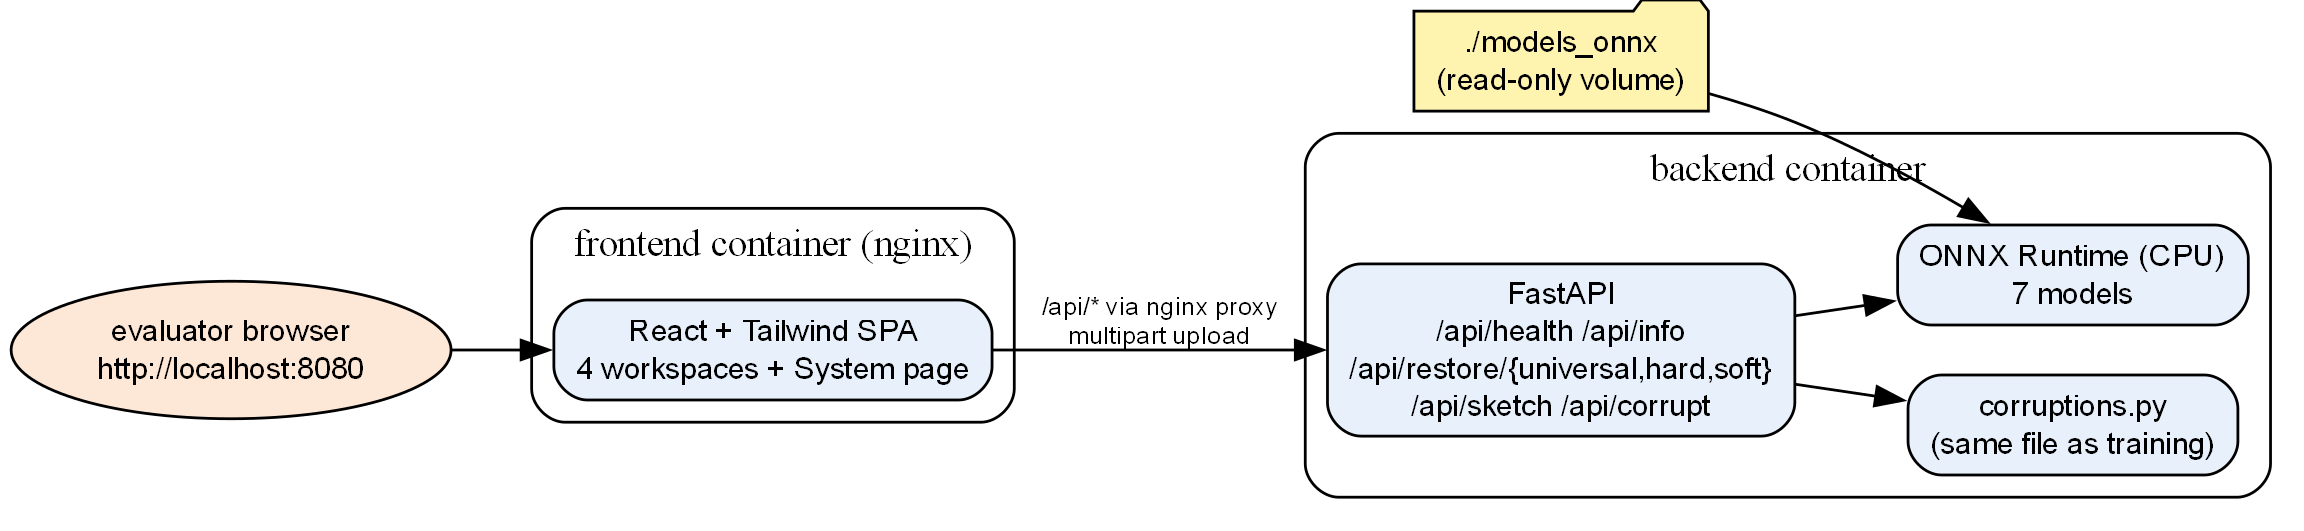
\includegraphics[width=\linewidth]{app.png}\caption{Deployment architecture.}\label{fig:apparch}\end{figure}}{}
\IfFileExists{figures/stitch_1.png}{\begin{figure}[t]\centering
\includegraphics[width=\linewidth]{stitch_1.png}\caption{Original Google Stitch design of the restoration workspace.}\label{fig:stitch}\end{figure}}{}
\IfFileExists{figures/app_hard.png}{\begin{figure}[t]\centering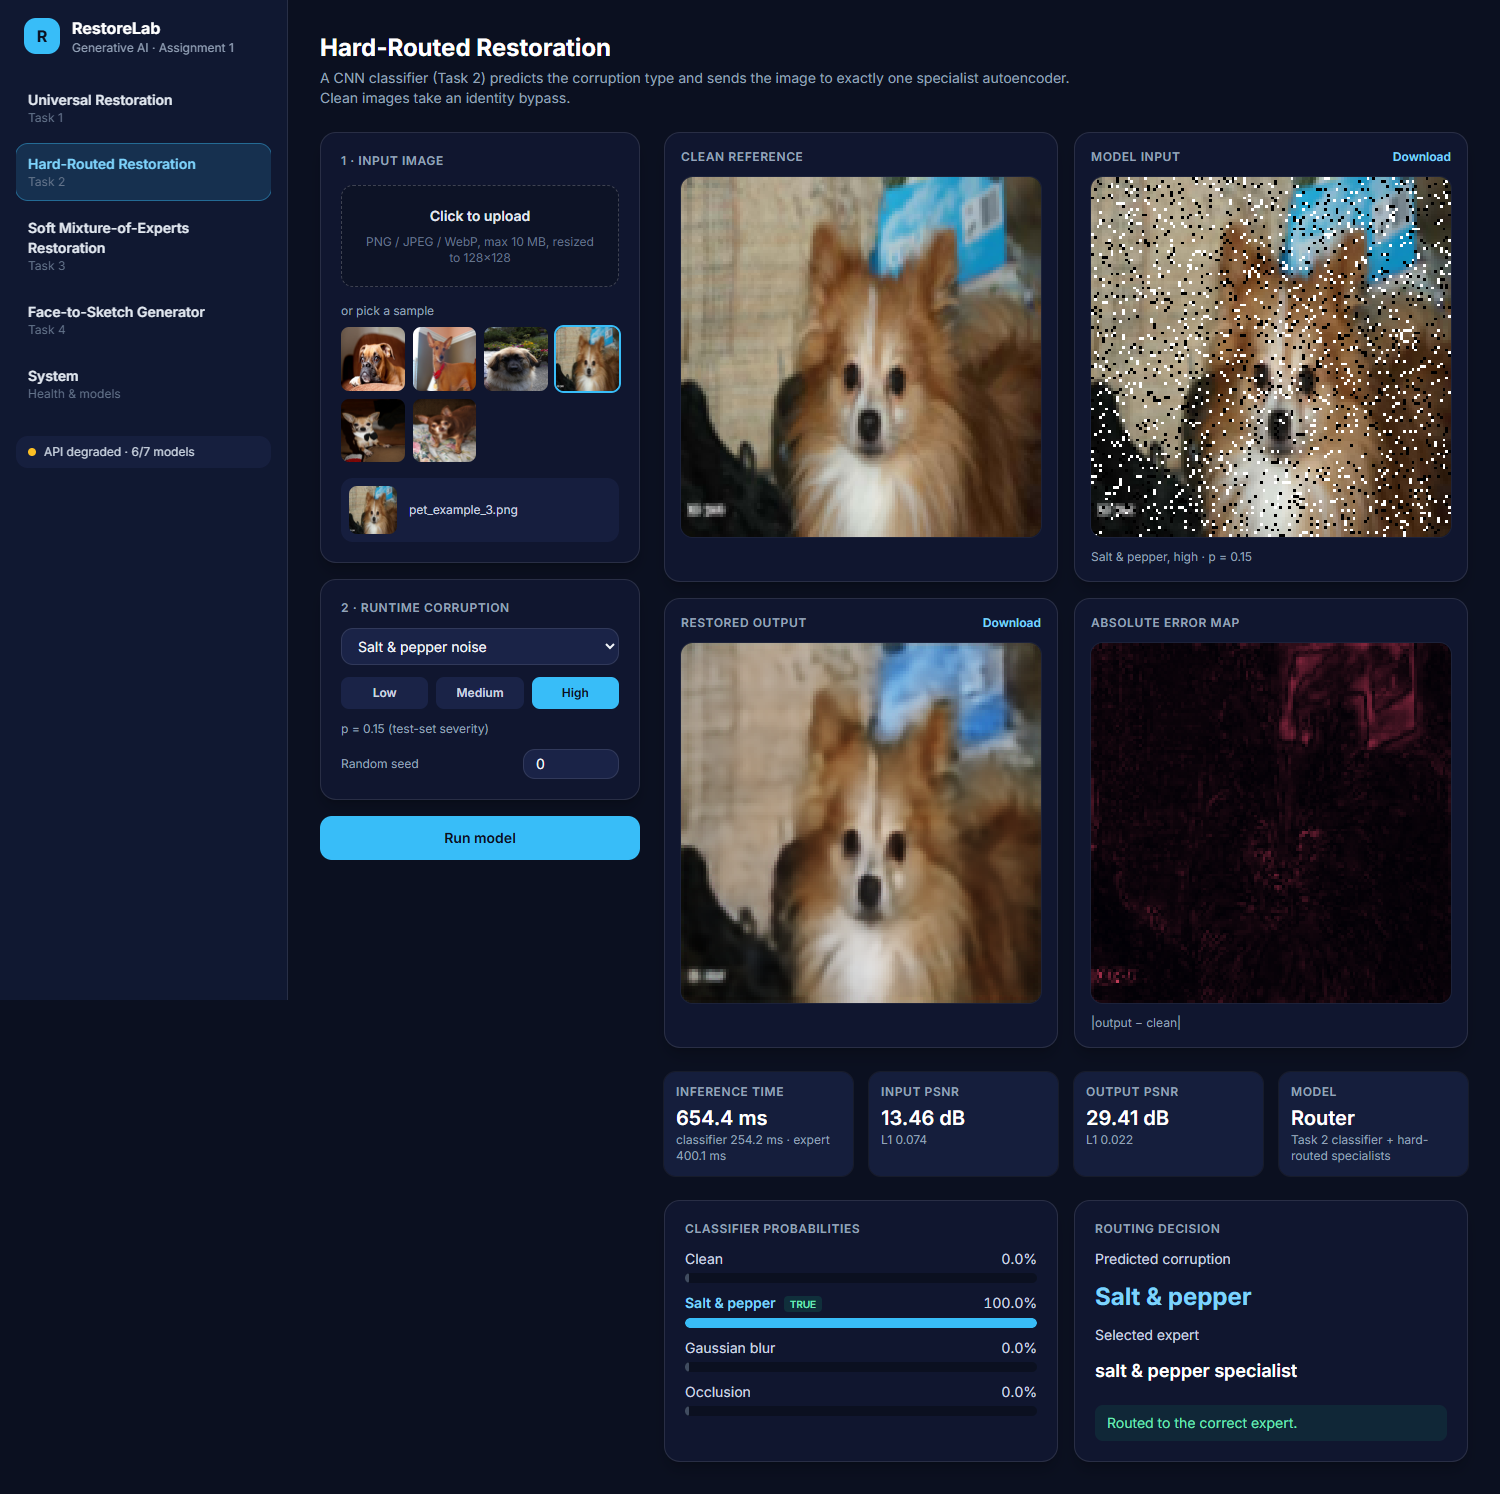
\includegraphics[width=\linewidth]{app_hard.png}\caption{Implemented Hard-Routed Restoration workspace (React + Tailwind).}\label{fig:app}\end{figure}}{}


\IfFileExists{figures/app_universal.png}{\begin{figure*}[t]\centering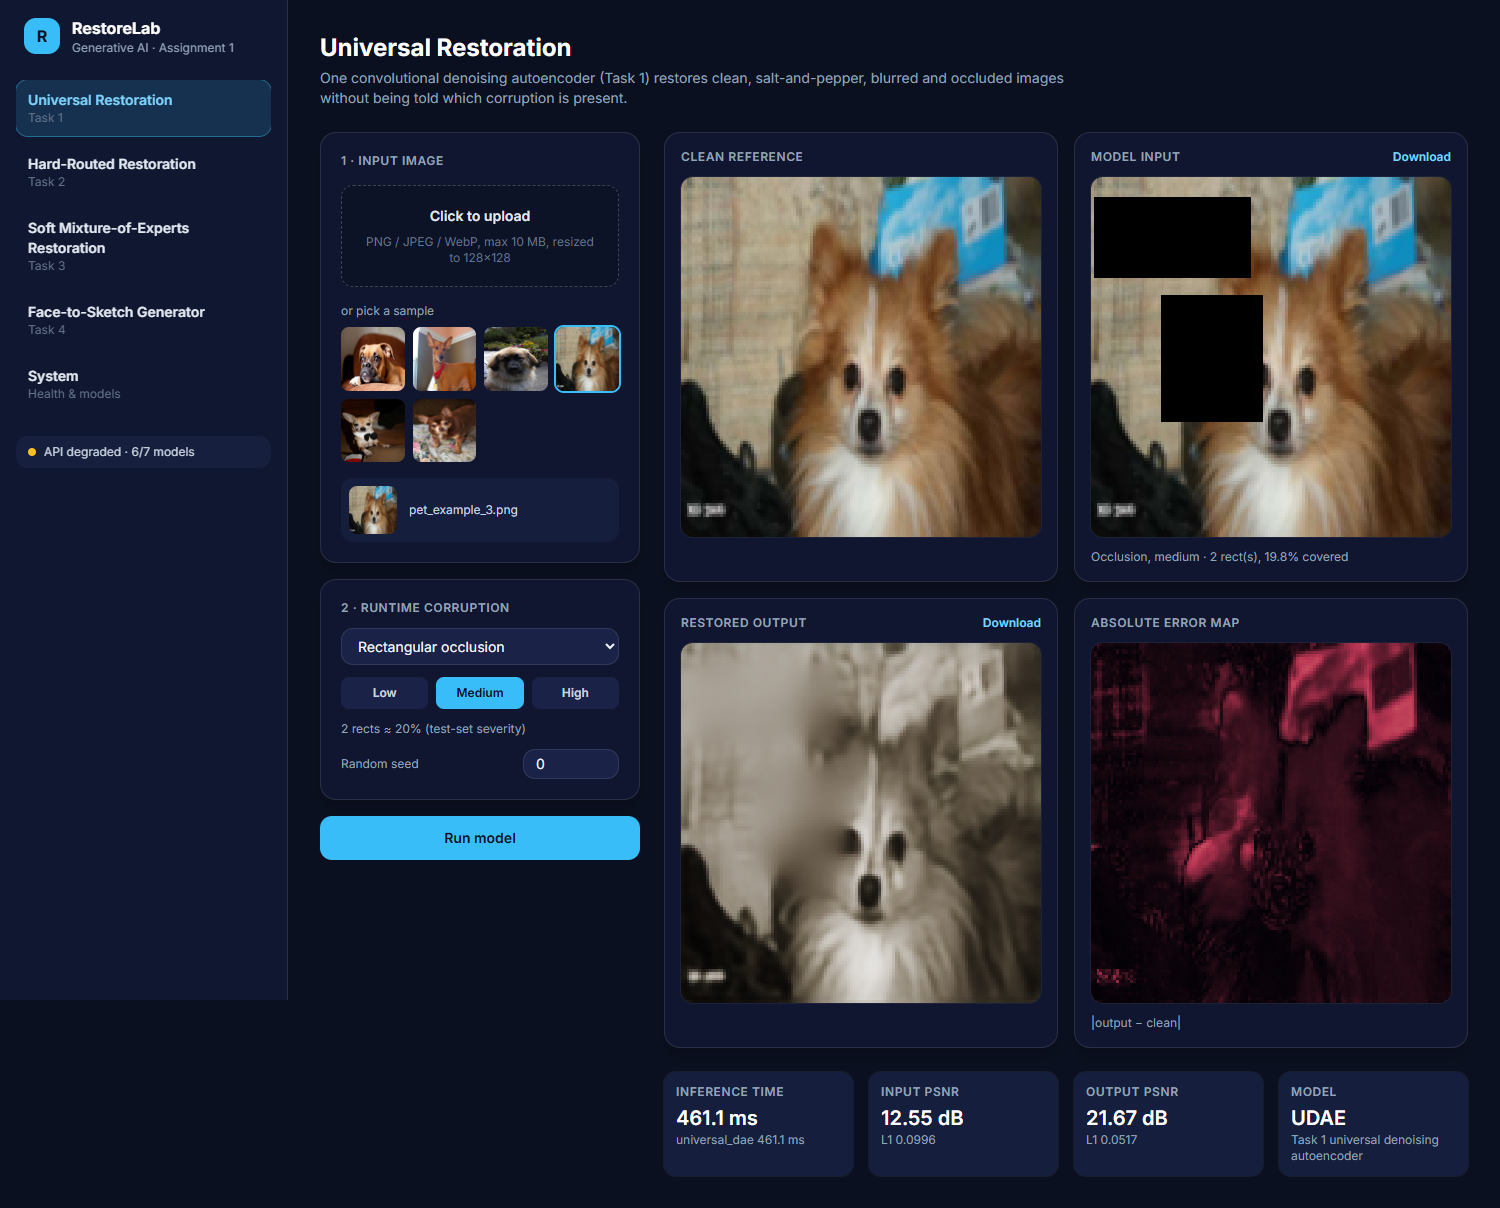
\includegraphics[width=0.32\linewidth]{app_universal.png}\hfill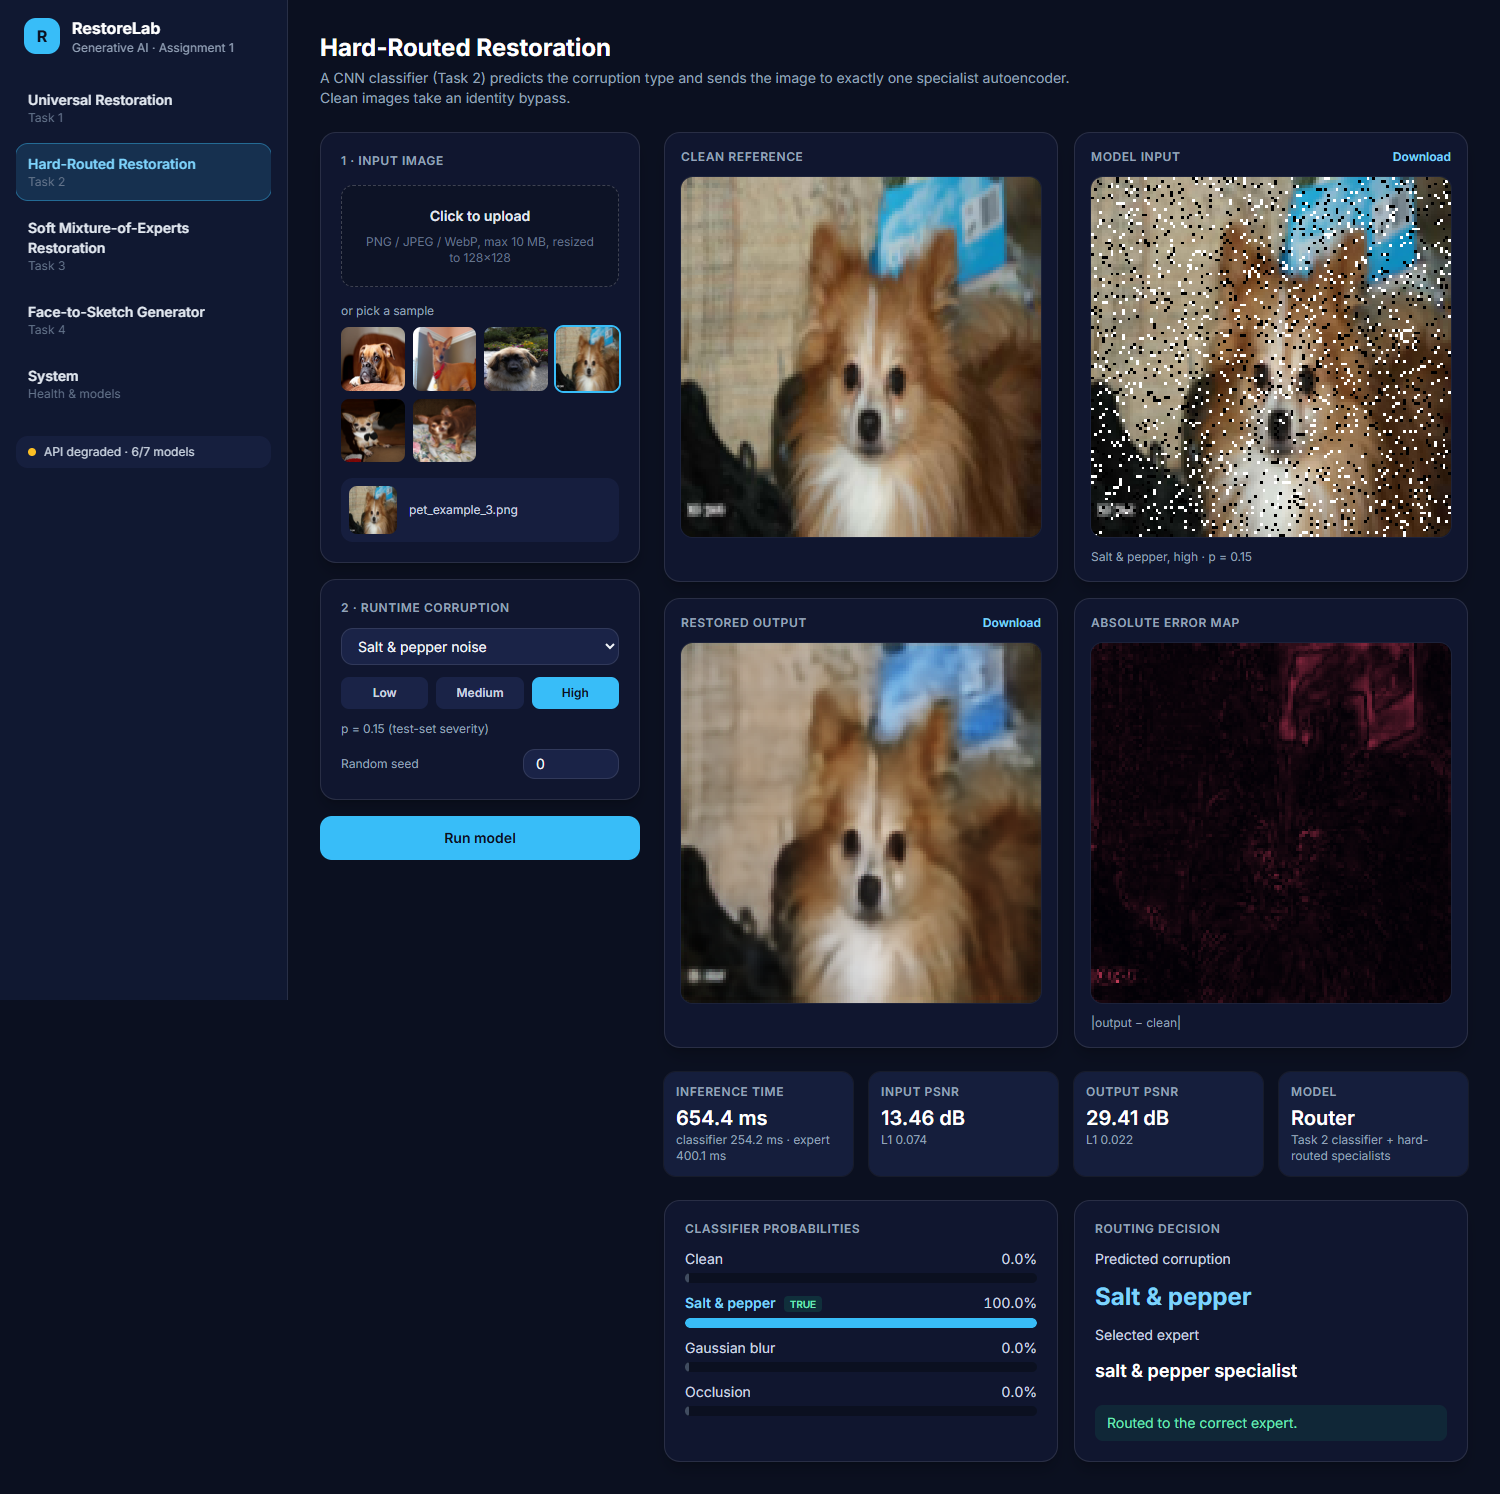
\includegraphics[width=0.32\linewidth]{app_hard.png}\hfill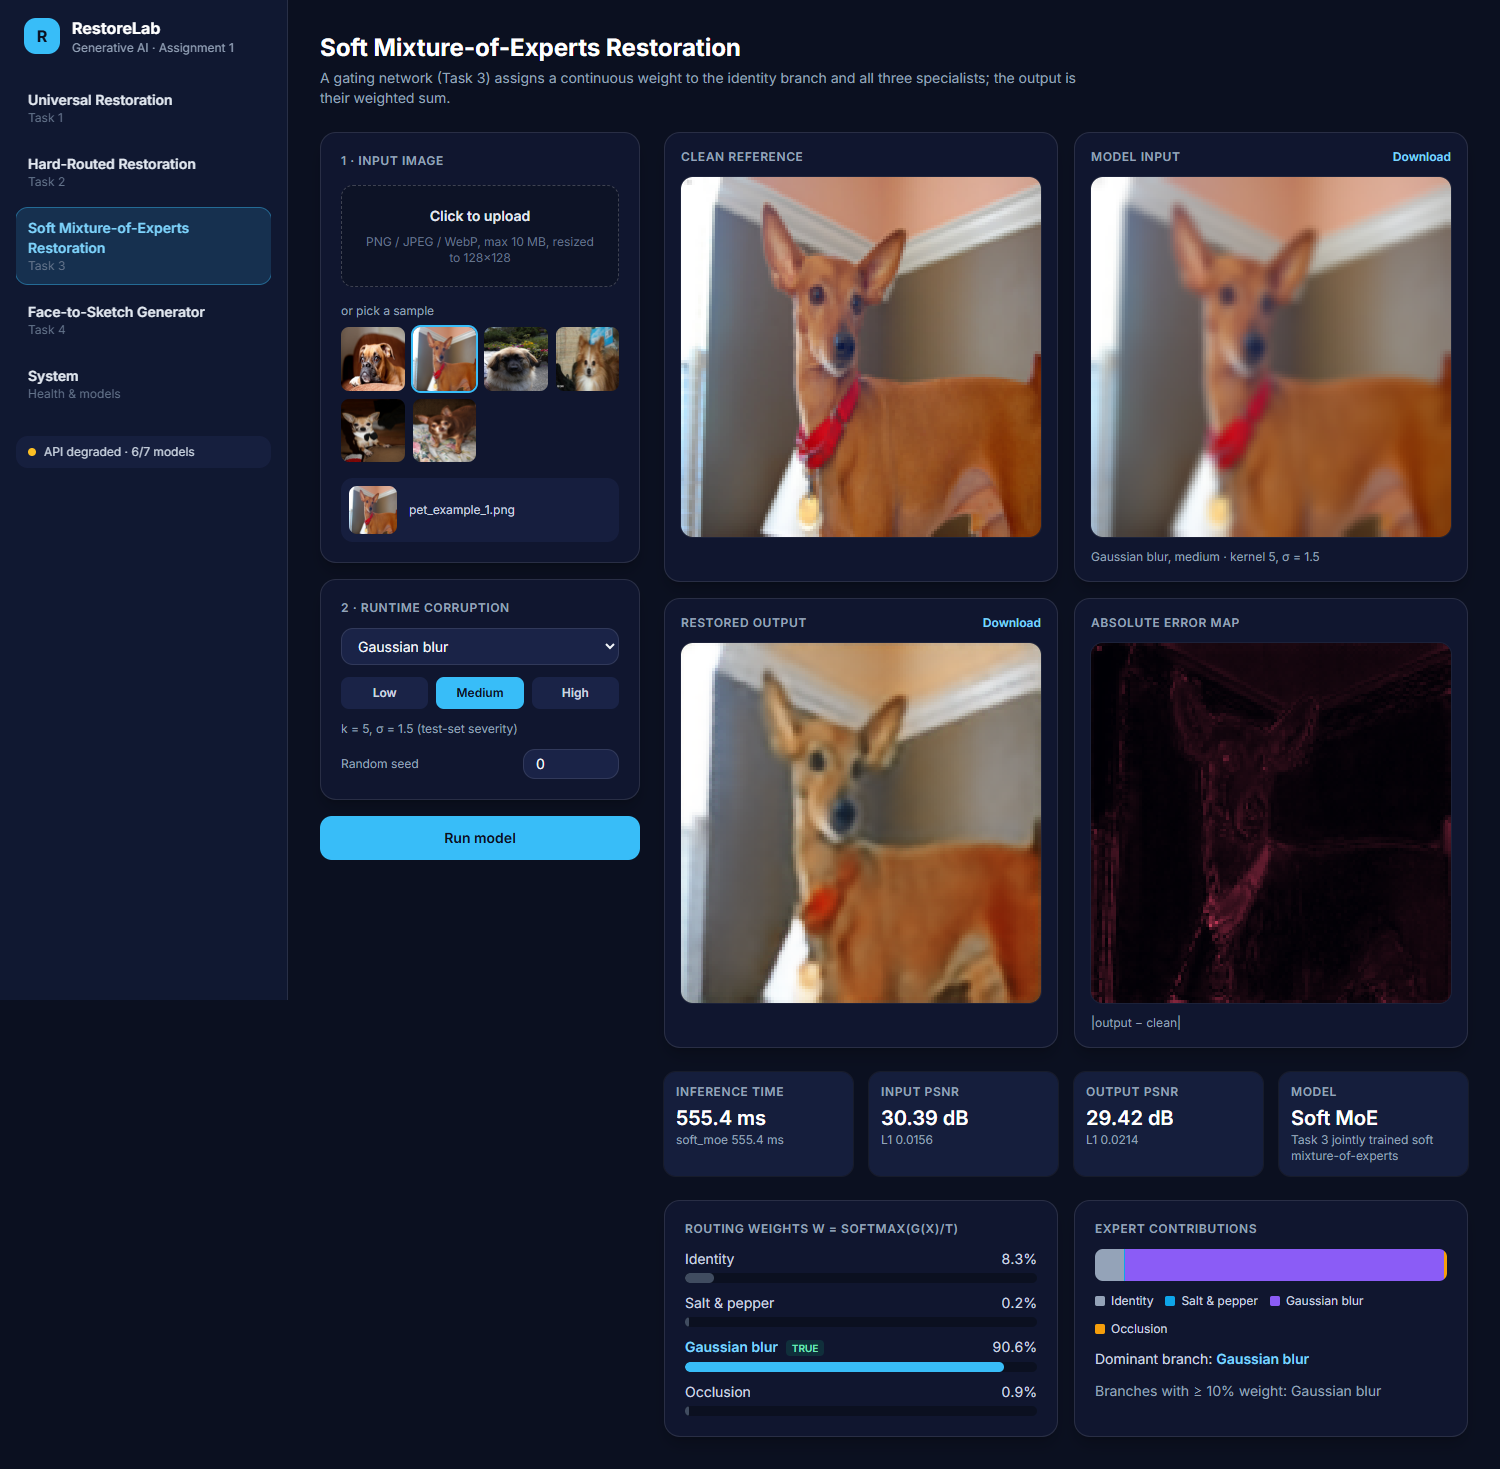
\includegraphics[width=0.32\linewidth]{app_soft.png}\caption{Application screenshots with the deployed ONNX models: Universal Restoration (occlusion, medium), Hard-Routed Restoration (salt-and-pepper; classifier probabilities and selected expert), Soft MoE Restoration (blur; 90.6\% weight on the blur expert).}\label{fig:appshots}\end{figure*}}{}
\IfFileExists{figures/app_sketch.png}{\begin{figure}[t]\centering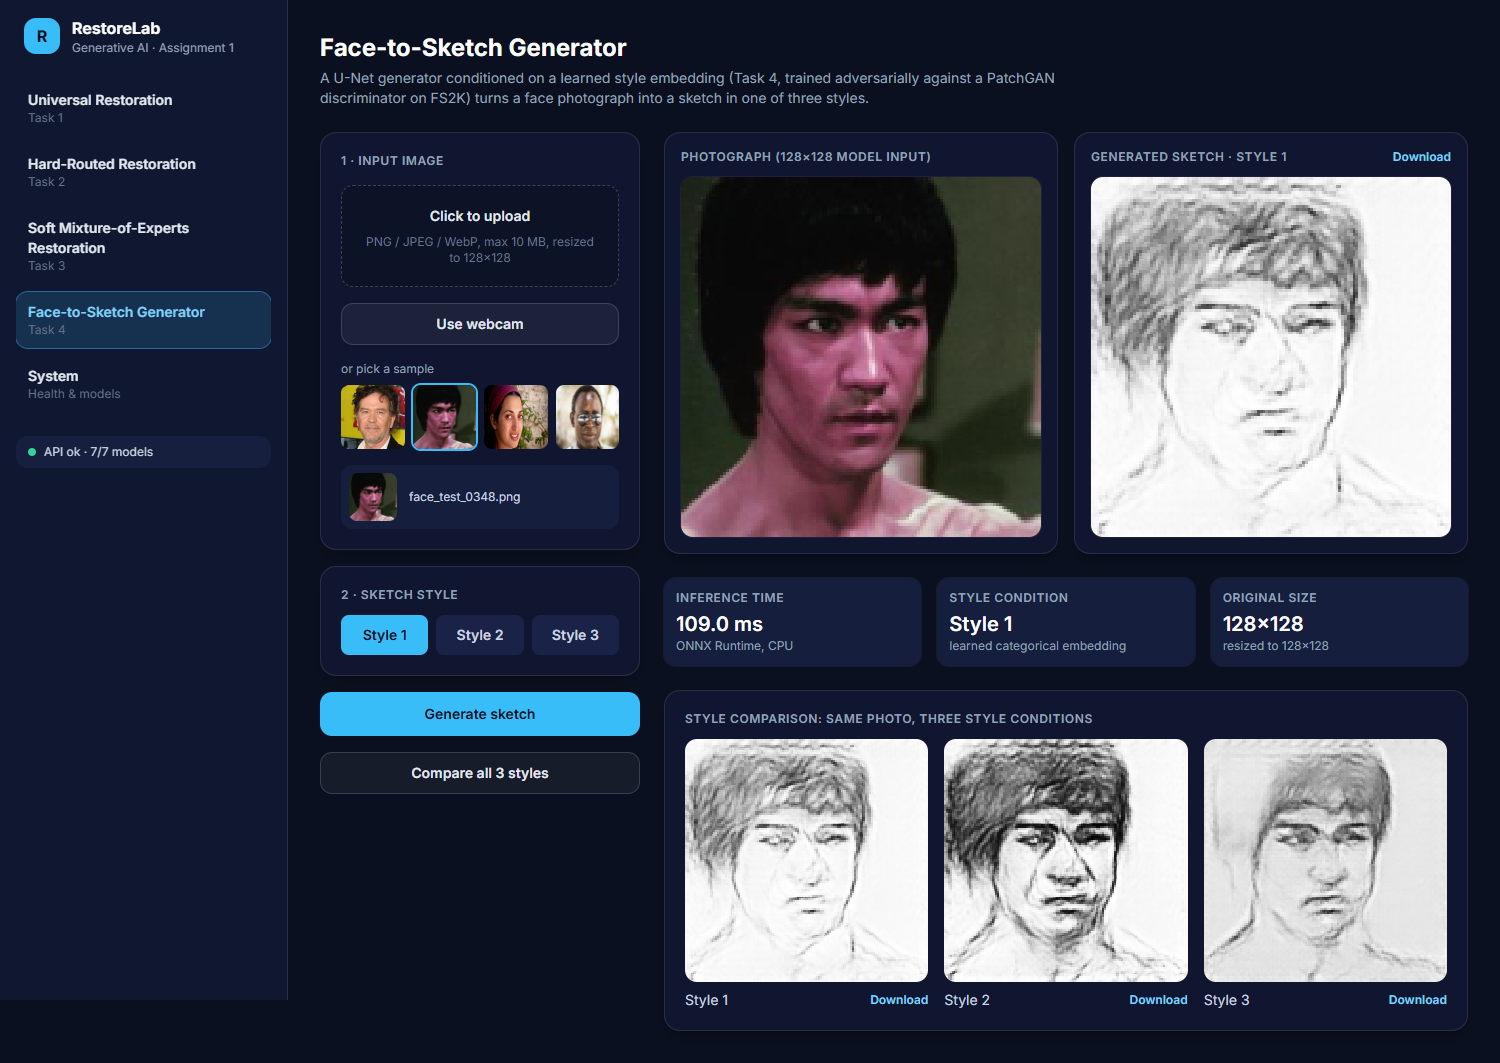
\includegraphics[width=\linewidth]{app_sketch.png}\caption{Face-to-Sketch Generator workspace: generated sketch and the three-style comparison for a test photograph.}\label{fig:appsketch}\end{figure}}{}
\IfFileExists{figures/app_system.png}{\begin{figure}[t]\centering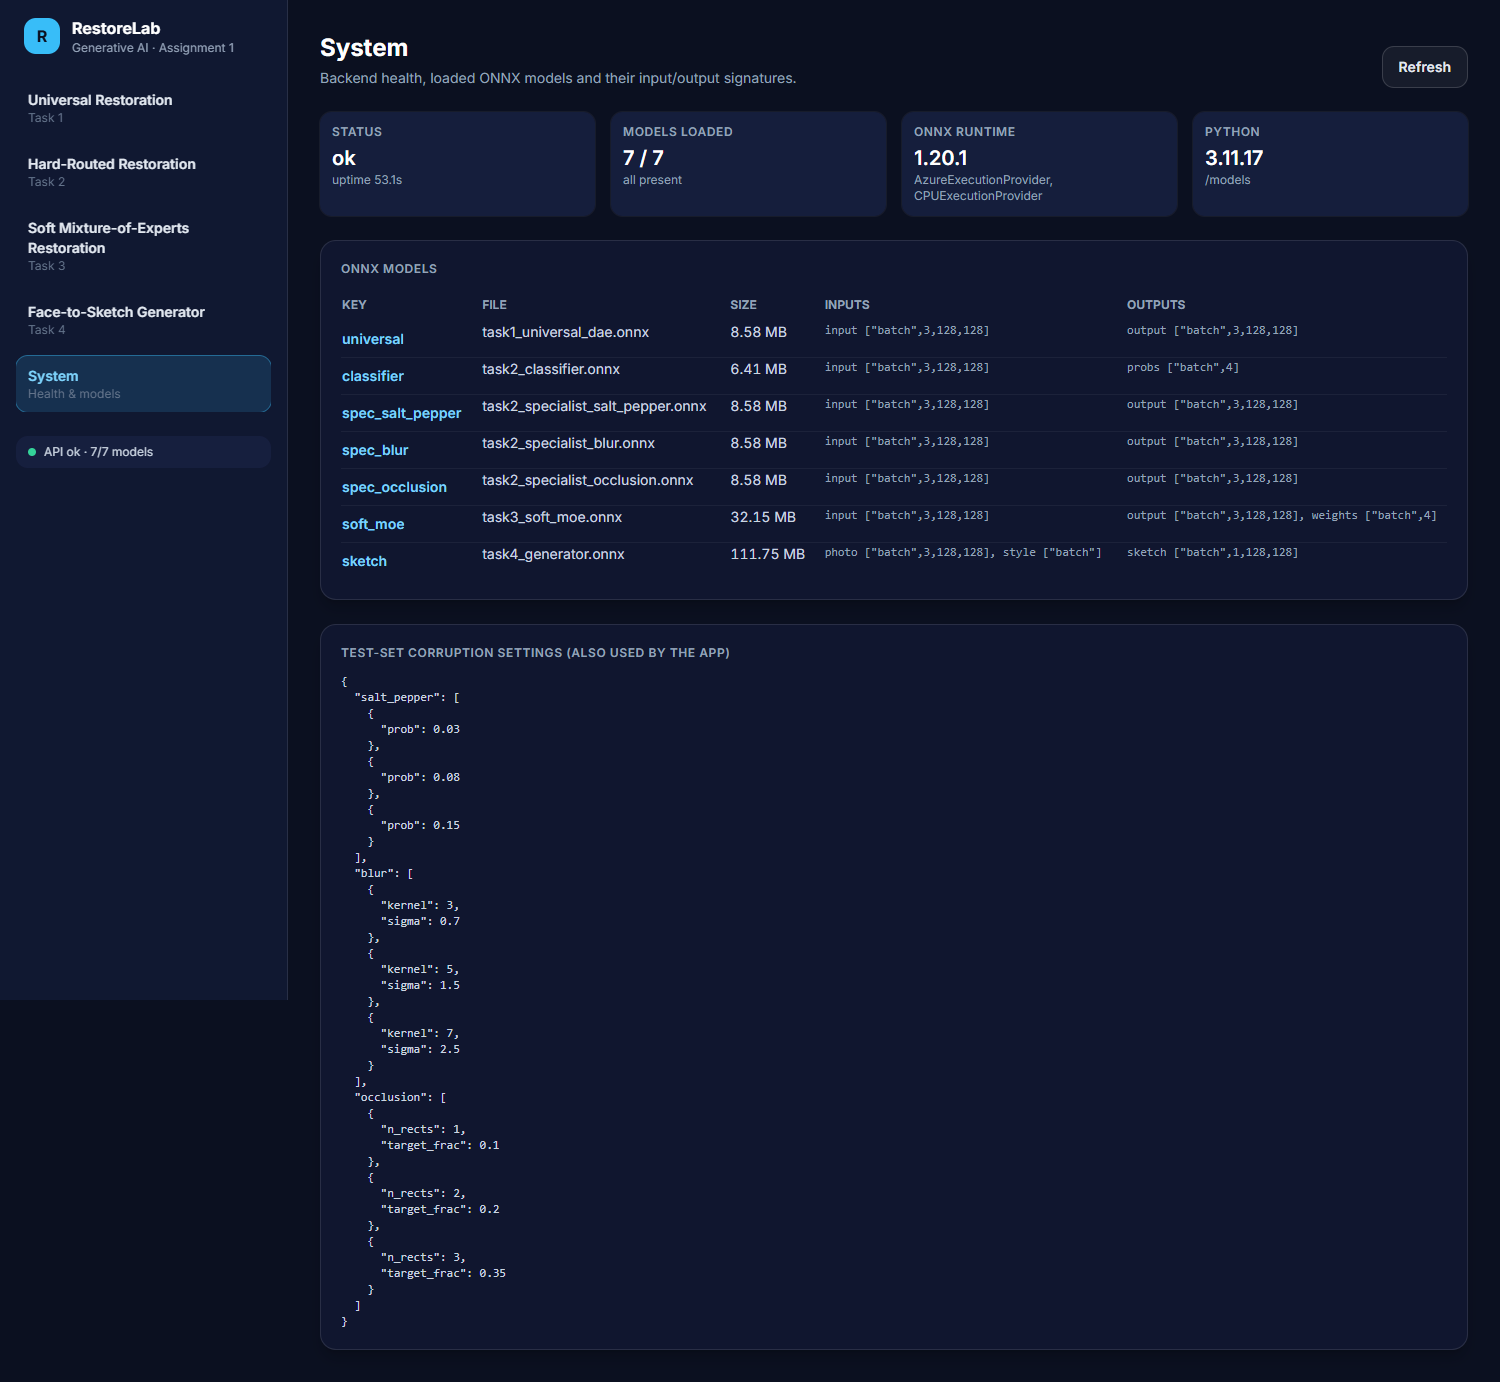
\includegraphics[width=\linewidth]{app_system.png}\caption{System page: loaded ONNX models and their signatures.}\label{fig:appsys}\end{figure}}{}

\section{Limitations}
(1) All models operate at $128\times128$, so fine fur texture is lost even by the best system. (2) Optuna budgets were small (4--12 trials, 4--8 epochs per trial) because of free-tier GPU limits, so the selected configurations are good rather than optimal, and short trials favour fast-converging settings. (3) The MoE gate is overconfident on corruption mixtures. (4) PSNR is capped at 50\,dB, which slightly flatters identity-branch results on clean images. (5) The Colab runtime disconnected twice; the resumable pipeline restored all completed stages from Drive, but the final Task~1 model came from a 12-trial study, and the Task~4 budget had to be reduced.

\section{Conclusion}
A single bottlenecked autoencoder removes heavy corruption but caps fidelity at about 23\,dB and damages clean inputs. Decomposing the problem into an accurate classifier (99.7\%) and specialists with an identity bypass improves PSNR by 5.3\,dB. Turning the router into a jointly fine-tuned soft MoE gives the best structural fidelity while learning interpretable, mostly sharp routing that blends branches where blending genuinely helps (small occlusions, blur). The style-conditioned cGAN shows clear, controllable style transfer but suffers from template artefacts on the hardest style. The main open problems are calibrated routing for unseen corruption mixtures and data-efficient sketch synthesis. All models run in a containerised web application from ONNX, with outputs matching PyTorch to within $1.1\cdot10^{-6}$.

\appendices
\section{AI-Use Statement}
\textbf{Tools.} Claude (Anthropic) was used as a coding and research assistant, and Google Stitch for the interface design. \textbf{Tasks.} Drafting the training, evaluation, export, backend and frontend code; suggesting the $\alpha$-independent Optuna objective, the PSNR cap and the class-balanced collate design; drafting the report structure and generating its LaTeX tables from our result files. \textbf{Verification.} Every script was first run end-to-end on synthetic data before training; five unit tests verify the corruption specification (ranges, salt/pepper split, occlusion coverage, determinism, blur equality with \texttt{torchvision}); ONNX outputs were compared numerically with PyTorch (max error $\le1.1\cdot10^{-6}$); the API was tested with valid and invalid uploads (415/422 responses); all numbers in this report are read from the CSV/JSON files produced by the scripts. \textbf{Corrections made during development.} A missing \texttt{load\_state\_dict} in evaluation, an ONNX check that sampled only clean images, an MLflow file store that newer MLflow refuses (switched to SQLite), PSNR overflow for identical images, CRLF line endings that broke the shell scripts on Linux, a PyTorch~2.6 checkpoint-loading change (\texttt{weights\_only}) that broke the Task~4 evaluation, and memory limits that required running training jobs sequentially.

\bibliographystyle{IEEEtran}
\begin{thebibliography}{99}
\bibitem{vincent2008} P.~Vincent, H.~Larochelle, Y.~Bengio and P.-A.~Manzagol, ``Extracting and composing robust features with denoising autoencoders,'' in \emph{Proc. ICML}, 2008.
\bibitem{mao2016} X.-J.~Mao, C.~Shen and Y.-B.~Yang, ``Image restoration using very deep convolutional encoder-decoder networks with symmetric skip connections,'' in \emph{Proc. NeurIPS}, 2016.
\bibitem{zhao2017} H.~Zhao, O.~Gallo, I.~Frosio and J.~Kautz, ``Loss functions for image restoration with neural networks,'' \emph{IEEE Trans. Comput. Imaging}, vol.~3, no.~1, 2017.
\bibitem{jacobs1991} R.~A.~Jacobs, M.~I.~Jordan, S.~J.~Nowlan and G.~E.~Hinton, ``Adaptive mixtures of local experts,'' \emph{Neural Computation}, vol.~3, no.~1, 1991.
\bibitem{shazeer2017} N.~Shazeer \emph{et al.}, ``Outrageously large neural networks: The sparsely-gated mixture-of-experts layer,'' in \emph{Proc. ICLR}, 2017.
\bibitem{fedus2022} W.~Fedus, B.~Zoph and N.~Shazeer, ``Switch Transformers: Scaling to trillion parameter models with simple and efficient sparsity,'' \emph{JMLR}, vol.~23, 2022.
\bibitem{isola2017} P.~Isola, J.-Y.~Zhu, T.~Zhou and A.~A.~Efros, ``Image-to-image translation with conditional adversarial networks,'' in \emph{Proc. CVPR}, 2017.
\bibitem{mirza2014} M.~Mirza and S.~Osindero, ``Conditional generative adversarial nets,'' arXiv:1411.1784, 2014.
\bibitem{miyato2018} T.~Miyato and M.~Koyama, ``cGANs with projection discriminator,'' in \emph{Proc. ICLR}, 2018.
\bibitem{fan2022} D.-P.~Fan \emph{et al.}, ``Facial-sketch synthesis: A new challenge,'' \emph{Machine Intelligence Research}, vol.~19, 2022.
\bibitem{akiba2019} T.~Akiba, S.~Sano, T.~Yanase, T.~Ohta and M.~Koyama, ``Optuna: A next-generation hyperparameter optimization framework,'' in \emph{Proc. KDD}, 2019.
\bibitem{parkhi2012} O.~M.~Parkhi, A.~Vedaldi, A.~Zisserman and C.~V.~Jawahar, ``Cats and dogs,'' in \emph{Proc. CVPR}, 2012.
\end{thebibliography}
\end{document}
